% \input{/Users/jovo/Research/latex/latex_paper.tex}

\documentclass[10pt,journal,cspaper,compsoc]{IEEEtran}
%
% If IEEEtran.cls has not been installed into the LaTeX system files,
% manually specify the path to it like:
% \documentclass[12pt,journal,compsoc]{../sty/IEEEtran}

\usepackage{fixltx2e}
% \usepackage{stfloats}
\usepackage{amsmath}
\usepackage{graphicx}
\usepackage{amsfonts}
\usepackage{amssymb}
\usepackage{amsthm}
\usepackage{cite}
\usepackage{algorithm}
\usepackage{algorithmic}
\usepackage{url}
\usepackage{enumerate}
% \usepackage{hyperref}
\usepackage{color}

\newcommand{\jv}{Joshua Vogelstein}
\newcommand{\jhu}{Johns Hopkins University}
%\newcommand{\hp}{https://jshare.johnshopkins.edu/jvogels3/public_html/}
\newcommand{\ema}{joshuav@jhu.edu}

\newcommand{\Vr}{V_{reset}}
\newcommand{\Vl}{V_{leat}}
\newcommand{\eqdef}{\overset{\triangle}{=}}
% \newcommand{\D}[2]{\frac{\partial #1}{\partial #2}}
\newcommand{\dd}[2]{\frac{\partial ^2 #1}{\partial #2 ^2}}
\newcommand{\DDD}[3]{\frac{\partial ^2 #1}{\partial #2 \partial #3}}
\newcommand{\Di}[2]{\frac{\partial ^i #1}{\partial #2 ^i}}
\newcommand{\grad}{\nabla}
\newcommand{\Hess}{\nabla\nabla}
\newcommand{\defn}{\overset{\triangle}{=}}

\providecommand{\tg}[1]{\textcolor{green}{#1}}
\providecommand{\tb}[1]{\textcolor{blue}{#1}}
\providecommand{\tr}[1]{\textcolor{red}{#1}}
\providecommand{\tk}[1]{\textcolor{black}{#1}}
\providecommand{\twhite}[1]{\textcolor{white}{#1}}
\providecommand{\ve}[1]{\boldsymbol{#1}}
\providecommand{\ma}[1]{\boldsymbol{#1}}
%\providecommand{\ve}[1]{\boldsymbol{#1}}
%\newcommand{\norm}[1]{\left|\left|#1\right|\right|}
\providecommand{\norm}[1]{\left \lVert#1 \right  \rVert}
\providecommand{\deter}[1]{\lvert #1 \rvert}
\providecommand{\abs}[1]{\left \lvert #1 \right \rvert}
\providecommand{\mat}[1]{\left[ #1 \right]}
\newcommand{\trans}[1]{{#1}^{\ensuremath{\mathsf{T}}}}           % transpose
\newcommand{\transpose}[1]{{#1}^{\ensuremath{\mathsf{T}}}}           % transpose
\newcommand{\argmax}{\operatornamewithlimits{argmax}}
\newcommand{\argmin}{\operatornamewithlimits{argmin}}
\newcommand{\T}{^{\ensuremath{\mathsf{T}}}}           % transpose
\newcommand{\from}{{\ensuremath{\colon}}}           % :

\newcommand{\Aa}{\mathbb{A}}
\newcommand{\BB}{\mathbb{B}}
\newcommand{\CC}{\mathbb{C}}         
\newcommand{\DD}{\mathbb{D}}         
\newcommand{\EE}{\mathbb{E}}           % expected value
\newcommand{\FF}{\mathbb{F}}         
\newcommand{\GG}{\mathbb{G}}
\newcommand{\HH}{\mathbb{H}}         
\newcommand{\II}{\mathbb{I}}           % indicator function
\newcommand{\LL}{\mathbb{L}}
\newcommand{\MM}{\mathbb{M}}
\newcommand{\NN}{\mathbb{N}}
\newcommand{\PP}{\mathbb{P}}         
\newcommand{\QQ}{\mathbb{Q}}           
\newcommand{\SSS}{\mathbb{S}}           
\newcommand{\VV}{\mathbb{V}}
\newcommand{\XX}{\mathbb{X}}         
\newcommand{\YY}{\mathbb{Y}}
\newcommand{\ZZ}{\mathbb{Z}}         

\newcommand{\iid}{\overset{iid}{\sim}}

% \DeclareMathOperator*{\argmax}{argmax}
% \DeclareMathOperator*{\argmin}{argmin}
% \DeclareMathOperator{\find}{find}

% \newtheorem{thm}{Theorem}
\newcommand{\thma}{\begin{thm}}
\newcommand{\thmb}{\end{thm}}

\newcommand{\mata}{\begin{bmatrix}}
\newcommand{\matb}{\end{bmatrix}}



\newtheorem{Rem}{Remark}%[section]
\newtheorem{Alg}{Algorithm}%[section]
\newtheorem{thm}{Theorem}
\newtheorem{lem}{Lemma}
\newtheorem{Thm}{Theorem}[section]
\newtheorem{Lem}{Lemma}%[section]
\newtheorem{defi}{Definition}
\newtheorem{Def}{Definition}[section]
\newtheorem{prop}{Proposition}
\newtheorem{coro}[thm]{Corollary}
\newtheorem{claim}{Claim}
\newtheorem{conj}{Conjecture}
\newtheorem{question}{Question}

% \newtheorem{corollary}{Corollary}
% \newtheorem{theorem}{Theorem}
%\theoremstyle{marginbreak}
%\newtheorem{Lem}[Cor]{Lemma}
%\theoremstyle{change}
%\theorembodyfont{\itshape}


% \newtheorem{defi}{Definition}
% \newcommand{\defa}{\begin{defi}}
% \newcommand{\defb}{\end{defi}}

% \newcommand{\eq}{\begin{equation}}
% \newcommand{\en}{\end{equation}}
% \newcommand{\eqa}{\begin{equation}}
% \newcommand{\eqb}{\end{equation}}

\newcommand{\enuma}{\begin{enumerate}}
\newcommand{\enumb}{\end{enumerate}}
\newcommand{\ena}{\begin{enumerate}}
\newcommand{\enb}{\end{enumerate}}

\newcommand{\itema}{\begin{itemize}}
\newcommand{\itemb}{\end{itemize}}
\newcommand{\ita}{\begin{itemize}}
\newcommand{\itb}{\end{itemize}}

% \newcommand{\aligna}{\begin{align}}
% \newcommand{\alignb}{\end{align}}

\newcommand{\proofa}{\begin{proof}}
\newcommand{\proofb}{\end{proof}}

\newcommand{\bla}{\begin{block}}
\newcommand{\blb}{\end{block}}

% \newcommand{\seqa}{\begin{equation*}}
\newcommand{\seqb}{\end{equation*}}

\newcommand{\bth}{\ve{\theta}}
\newcommand{\hth}{\mh{\theta}}
\newcommand{\htth}{\mh{\theta}}
\newcommand{\bhth}{\mh{\ve{\theta}}}
\newcommand{\thetn}{\ve{\theta}}
\newcommand{\thet}{\thetn}
\newcommand{\theth}{\widehat{\ve{\theta}}}
\newcommand{\theto}{\ve{\theta}'}
\newcommand{\wht}{\widehat{\thet}}
\newcommand{\wtt}{\widetilde{\thet}}
\newcommand{\vth}{\ve{\thet}}
\newcommand{\vTh}{\ve{\Theta}}
\newcommand{\hvth}{\widehat{\ve{\thet}}}
\newcommand{\bTh}{\ve{\Theta}}
\newcommand{\hbth}{\widehat{\thet}}

% \newcommand{\p}{P_{\bth}}
\newcommand{\pold}{P_{\bth'}}
\newcommand{\pk}{P_{\widehat{\ve{\theta}}^{(k)}}}
\newcommand{\pT}{P_{\thetn_{Tr}}} %\thetn_T
\newcommand{\pO}{P_{\thetn_o}} %\thetn_o
% \newcommand{\Q}{Q(\thetn,\theto)}
% \newcommand{\m}{m^{\ast}}
% \newcommand{\q}{q(\ve{H}_t)}
\newcommand{\Ca}{[\text{Ca}^{2+}]}

\newcommand{\Lik}{\mathcal{L}}
\newcommand{\Cae}{[\widehat{\text{Ca}}^{2+}]}
\newcommand{\Cav}{\ve{C}}%[\ve{\text{Ca}}^{2+}]}
\newcommand{\sml}{\sqrt{\ma{\lambda}}}
\newcommand{\ml}{\ma{\lambda}}
\newcommand{\nw}{\widehat{n}}
\newcommand{\nv}{\vec{n}}
\newcommand{\Ae}{\widehat{A}}
\newcommand{\te}{\widehat{\tau}}
\newcommand{\maxn}{\max_{\ve{n}: n_t \geq 0}}
% \newcommand{\V}{\text{Var}}

\providecommand{\ms}[1]{\mathsf{#1}}
\providecommand{\mc}[1]{\mathcal{#1}}
\providecommand{\mb}[1]{\boldsymbol{#1}}
\providecommand{\mbb}[1]{\mathbb{#1}}
\providecommand{\mv}[1]{\vec{#1}}
\providecommand{\mh}[1]{\hat{#1}}
\providecommand{\wh}[1]{\widehat{#1}}
\providecommand{\mhv}[1]{\mh{\mv{#1}}}
\providecommand{\mvh}[1]{\mv{\mh{#1}}}
\providecommand{\mt}[1]{\widetilde{#1}}
\providecommand{\mhc}[1]{\hat{\mathcal{#1}}}
\providecommand{\mbc}[1]{\mb{\mathcal{#1}}}
\providecommand{\mvc}[1]{\mv{\mathcal{#1}}}
\providecommand{\mtc}[1]{\widetilde{\mathcal{#1}}}
\providecommand{\mhb}[1]{\hat{\boldsymbol{#1}}}
\providecommand{\whb}[1]{\widehat{\boldsymbol{#1}}}
\providecommand{\mvb}[1]{\vec{\boldsymbol{#1}}}
\providecommand{\mtb}[1]{\widetilde{\boldsymbol{#1}}}

\newcommand{\mP}{\mathbb{P}}

\newcommand{\del}{\delta}
\newcommand{\sig}{\sigma}
\newcommand{\lam}{\lambda}
\newcommand{\gam}{\gamma}
\newcommand{\eps}{\varepsilon}

\newcommand{\Del}{\Delta}
\newcommand{\Sig}{\Sigma}
\newcommand{\Lam}{\Lambda}
\newcommand{\Gam}{\Gamma}

\newcommand{\dvs}{\dot{\bs}_t}
\newcommand{\dvw}{\dot{\bw}_t}
\newcommand{\dvx}{\dot{\bx}_t}
\newcommand{\dvy}{\dot{\by}_t}

\newcommand{\ft}{f_{\ve{\thet}}}
\newcommand{\gt}{g_{\ve{\thet}}}
\newcommand{\hht}{h_{\thetn}}

\newcommand{\Real}{\mathbb{R}}

\newcommand{\wconv}{\overset{i.p.}{\rightarrow}}
\newcommand{\sconv}{\overset{i.p.}{\rightarrow}}
\newcommand{\conv}{\rightarrow}
\newcommand{\pconv}{\overset{p}{\conv}}
\newcommand{\mcE}{\mathcal{E}}
\newcommand{\mcT}{\mathcal{T}}
\newcommand{\mcG}{\mathcal{G}}
\newcommand{\mcM}{\mathcal{M}}
\newcommand{\mcL}{\mathcal{L}}
\newcommand{\hatmcE}{\widehat{\mcE}}
\newcommand{\hatp}{\widehat{p}}
\newcommand{\hatP}{\widehat{P}}
\newcommand{\hatQ}{\widehat{Q}}
\newcommand{\hatL}{\widehat{L}}
\newcommand{\mhP}{\widehat{\PP}}
\newcommand{\tildeA}{\widetilde{A}}

\newcommand{\defa}{\begin{defi}}
\newcommand{\defb}{\end{defi}}
\newcommand{\defeq}{\overset{\triangle}{=}}


% \renewcommand{\algorithmicrequire}{\textbf{Input:}}
% \renewcommand{\algorithmicensure}{\textbf{Output:}}



% \newcommand{\ss}{\mc{S}}
% \newcommand{\mhc}{\mh{\mc{S}}_n}

% \newcommand{\Real}{\mathbb{R}}
% \newcommand{\bTh}{\mb{\Theta}}
% \newcommand{\ra}{\rightarrow}
% \newcommand{\la}{\leftarrow}
\newcommand{\bX}{\mb{X}}

% \newcommand{\bv}{\mb{v}}
% \newcommand{\ba}{\mb{a}}
% \newcommand{\bd}{\mb{d}}
% \newcommand{\balpha}{\mb{\alpha}}
% \newcommand{\conv}{\rightarrow}  
% \newcommand{\xx}{\langle \bx_u^\la, \bx_v^\ra\rangle}  
% \DeclareMathOperator*{\argmax}{arg \hspace{1pt} max \hspace{2pt}}
% \DeclareMathOperator*{\argmin}{arg \hspace{1pt} min \hspace{2pt}}
% \newcommand{\norm}[1]{\left \lVert#1 \right  \rVert}
% 


\newcommand{\theHalgorithm}{\arabic{algorithm}}


\DeclareMathOperator{\Delti}{\mathbf{\Delta}^{-1}}
\DeclareMathOperator{\Delt}{Q} %\mathbf{\Delta}}
% \DeclareMathOperator{\Gam}{\mathbf{\Gamma}}
\DeclareMathOperator{\Gami}{\mathbf{\Gamma}^{-1}}
\DeclareMathOperator{\Sigb}{\mathbf{\Sigma}}
\DeclareMathOperator{\Ri}{\mathbf{\R}^{-1}}
\DeclareMathOperator{\A}{A}
\DeclareMathOperator{\W}{\mathbf{W}}
\DeclareMathOperator{\V}{\mathbf{V}}
\DeclareMathOperator{\U}{\mathbf{U}}
\DeclareMathOperator{\C}{\mathbf{C}}
\DeclareMathOperator{\uvec}{\mathbf{u}}
\DeclareMathOperator{\D}{\mathbf{D}}
\DeclareMathOperator{\Q}{\mathbf{Q}}
\DeclareMathOperator{\R}{R} %\mathbf{P}}
\DeclareMathOperator{\Y}{\mathbf{Y}}
\DeclareMathOperator{\B}{\mathbf{B}}
\DeclareMathOperator{\Hmat}{\mathbf{H}}
\DeclareMathOperator{\Gmat}{\mathbf{G}}
\DeclareMathOperator{\X}{\mathbf{X}}
\DeclareMathOperator{\Cmat}{C} %\mathbf{L}}
\DeclareMathOperator{\Pmat}{\mathbf{P}}
\DeclareMathOperator{\veta}{\mathbf{\mb{v}}}
\DeclareMathOperator*{\minimize}{\mathrm{minimize}}
\DeclareMathOperator*{\maximize}{\mathrm{maximize}}
\DeclareMathOperator*{\Ymod}{\mathbf{\Y}}
\DeclareMathOperator*{\Bmod}{\mathbf{B}}
\DeclareMathOperator*{\Hmod}{\mathbf{H}}
\DeclareMathOperator*{\Lmod}{\mathbf{L}}
\DeclareMathOperator*{\Xmod}{\mathbf{\X}}
% \DeclareMathOperator*{\mb{v}mod}{\mathbf{\mb{v}}}

\newcommand{\elegans}{\emph{C. elegans} }

\newcommand{\FAQ}{\texttt{FAQ} }

\providecommand{\tg}[1]{\textcolor{green}{#1}}
\providecommand{\tb}[1]{\textcolor{blue}{#1}}
\providecommand{\tr}[1]{\textcolor{red}{#1}}



% \newcommand{\texttt{PATH}}{\texttt{PATH}}



\hyphenation{op-tical net-works semi-conduc-tor}
% \newcommand{\Qqap}{\Qqap}
\usepackage{caption}
\captionsetup{justification=raggedright}
\newcommand{\PmcP}{P \in \mc{P}}


\begin{document}

\title{(Brain) Graph Matching via \\ Fast Approximate Quadratic Programming}

% \huge{A Fast Approximate Quadratic Assignment Problem Algorithm for Brain Graph Matching}} % \\ with Applications in Statistical Connectomics}
% \title{A Quadratic Assignment Problem Approach to Graph Matching: Applications in Statistical Connectomics}

\author{Joshua T.~Vogelstein, John M.~Conroy, Louis J.~Podrazik, Steven G.~Kratzer, Eric T.~Harley,
        Donniell E.~Fishkind, 
		R.~Jacob~Vogelstein,
        and~Carey~E.~Priebe% <-this % stops a space
\IEEEcompsocitemizethanks{\IEEEcompsocthanksitem J.T. Vogelstein, D.E. Fishkind, and C.E. Priebe are with the Department
of Applied Mathematics and Statistics, Johns Hopkins University, Baltimore, MD 21218. 
%\protect\\
% note need leading \protect in front of \\ to get a newline within \thanks as
% \\ is fragile and will error, could use \hfil\break instead.
E-mail: \{joshuav,def,cep\}@jhu.edu, \{conroyjohnm,ljpodra,sgkratz\}@gmail.com, jacob.vogelstein@jhuapl.edu
\IEEEcompsocthanksitem J.M. Conroy, L.J. Podrazik and S.G. Kratzer are with Institute for Defense Analyses, Center for Computing Sciences, Bowie, MD 20708.
\IEEEcompsocthanksitem R.J. Vogelstein is with the Johns Hopkins University Applied Physics Laboratory, Laurel, MD, 20723.}% <-this % stops a space
\thanks{This work was partially supported by the Research Program in Applied Neuroscience.}}
 
% The paper headers
\markboth{SUBMITTED}
{Fast Inexact Graph Matching}

\IEEEcompsoctitleabstractindextext{%
\begin{abstract}
	
Graph matching (GM)---the process of finding an optimal permutation of the vertices of one graph to minimize adjacency disagreements with the vertices of another---is rapidly becoming an increasingly important computational problem, arising in fields ranging from machine vision to chemical engineering to neuroscience. Because GM is NP-hard, exact algorithms are unsuitable for today's massive graphs; yet, scalable GM algorithms have received short shrift.  GM can be formulated as a quadratic program with linear and binary constraints.  We develop a fast approximate quadratic (\FAQ) assignment algorithm to approximately solve a relaxed quadratic program with only linear constraints.  \FAQ scales cubicly with the number of vertices, and demonstrates marked improvements over previous state-of-the-art on nearly all benchmarks. Moreover, our non-convex formulation facilitates multiple restarts; $2-3$ wisely chosen initial conditions yield the best objective function on \emph{all} benchmarks. We find qualitatively similar results for our motivating application: brain-graph matching.  Unfortunately, the computational complexity of \FAQ scales too poorly to use it for mammalian brain-graphs, with millions or billions of vertices.  To inspire further development of approximate solutions to these problems, this work is available from on the first author's website, \url{http://jovo.me}.


% The quadratic assignment problem (QAP) arises in numerous disparate applications, ranging from traveling salesman problems to various machine vision problems.  We are particularly interested in a special case of QAP often called the (weighted) graph matching problem---the process of determining which permutation assigns vertices of one graph to those of another. 
% Our work is motivated by a particular graph matching problem: 
% Unfortunately, FAQ does not scale up to graphs with millions or billions of vertices, the size of mammalian brain-graphs.  
% A brain-graph (or connectome), is a graph in which vertices correspond to (collections of) neurons, and edges are either functional or structural connections between them.  
% % that is matching one connectome (brain-graph) to another. We are further interested in a specific application of graph matching applied to ``connectomes'' (networks comprising whole brains), which we call \emph{brain-graph matching}.  
% Brain-graphs have between $n \dot{\approx} 10^2$ and $\dot{\approx} 10^{11}$ vertices, making exact graph matching algorithms computationally infeasible, even for the smallest brains.  We cast our brain-graph matching problem as a nonlinearly constrained quadratic program.  Relaxing the constraints yields a simpler quadratic problem with linear constraints.  Our Fast Approximate Quadratic Assignment Problem algorithm, \texttt{FAQ}, finds a local minimum of this problem in $\mc{O}(n^3)$ time, outperforming the current state-of-the-art inexact (heuristic) algorithms on a number of QAP benchmarks.  Moreover, we prove that our relaxed optimization function has the same solution as the original problem in certain scenarios. Applying \texttt{FAQ} to a synthetic \emph{Caenorhabditis elegans} connectome problem demonstrates that brain-graph matching is much more difficult than many standard QAP benchmarks.  Utilizing multiple random restarts, however, often yields optimal performance on this task with $\dot{\approx} 300$ vertices.  
% .  To that end, 
% , and share our code 
% The formalism and algorithm we utilize here are designed for extending performance on larger and more complicated QAPs. 


 % This work presents an inexact strategy for GM.  Specifically, we frame GM as a quadratic assignment problem, and then relax the feasible region to its convex hull.  We prove that our relaxed optimization function has the same solution as the original problem, yet it is continuously differentiable. Because the objective function is not necessarily convex, we consider multiple principled initializations.  Performance exceeds the previous state-of-the-art in \emph{all} of 16 benchmark tests.  Moreover, this approach is fast, scaling cubically with the number of vertices, requiring only about a minute on a laptop for graphs with a few hundred vertices.  We illustrate this approach via a brain-graph application (the Caenorhabditis elegans ``connectome'').  We find that we can find the optimal solution for nearly every random permutation of the connectome that we sample.  Although this strategy already natively operates on weighted graphs, either directed or undirected, we propose a number of possible extensions, and make all code available.
\end{abstract}

% Note that keywords are not normally used for peer review papers.
\begin{keywords}
graph theory, network theory, statistical inference, structural pattern recognition, connectome.
\end{keywords}}


% make the title area
\maketitle
\IEEEdisplaynotcompsoctitleabstractindextext
\IEEEpeerreviewmaketitle



\section{Introduction}

\IEEEPARstart{G}{raph} matching---the process of finding an optimal permutation of the vertices of one graph to minimize adjacency disagreements with the vertices of another---is a famously computationally daunting problem (see, for example, ``Thirty Years of Graph Matching in Pattern Recognition''  \cite{Conte2004}). Specifically, graph matching is an $\mc{NP}$-hard problem, in particular, we do not know whether a polynomial time algorithm can solve it \cite{Papadimitriou1998}.  Perhaps the most prominent special case of graph matching is the traveling salesman problem \cite{Burkard2009}. As such, performance of graph matching algorithms are usually evaluated on graphs with $\dot{\approx} 10$ vertices, or at maximum $\dot{\approx} 100$ (see \cite{Burkard1997} for a description of the standard set of benchmarks).  Yet, it is increasingly popular to represent large data sets by a graph, and thus increasingly desirable to consider matching large graphs.  

The motivating application for this work is \emph{brain-graph matching}.  A brain-graph (aka, a connectome) is a graph for which vertices represent (collections of) neurons and edges represent connections between them \cite{SpornsKotter05, Hagmann05}. Via  Magnetic resonance (MR) imaging, one can image the whole brain and estimate connectivity across voxels, yielding a voxelwise connectome with up to $\dot{\approx} 10^6$ vertices and $\dot{\approx} 10^9$ edges \cite{Zuo2011}.  Comparing brains is an important step for many neurobiological inference tasks.  For example, it is becoming increasingly popular to diagnose neurological diseases via comparing brain images \cite{Csernansky2004}.  To date, however, these comparisons have largely rested on anatomical (e.g., shape) comparisons, not graph comparisons.  This is despite the widely held doctrine that many
% Yet almost immediately after the ``neuron doctrine'' was conjectured (the idea that networks of neurons comprise brains), Wernicke and others began postulating that 
psychiatric disorders are fundamentally ``connectopathies'', that is, disorders of the connections of the brain \cite{Kubicki2007,Calhoun2011,Fornito2012,Fornito2012a}. Currently available tests for connectopic explanation of psychiatric disorders  hedge upon first choosing some number of graph invariants to compare across populations. The graph invariant approach to classifying is both theoretically and practically inferior to comparing whole graphs via matching \cite{VP11_unlabeled}.  

More generally, state-of-the-art inference procedures for essentially any decision-theoretic or inference task follow from constructing interpoint dissimilarity matrices \cite{Duin2011}.  Thus, we believe that graph matching of large graphs will become a fundamental subroutine of many statistical inference pipelines operating on graphs. Because the number of vertices of these graphs is so large, exact matching is intractable.   Instead, we require inexact matching algorithms (also called ``heuristics'') that will scale polynomially or even linear \cite{Conte2004}.  We develop an approach to graph matching based on a relaxation of the quadratic programming problem (QAP).  Our approach is only cubic in the number of vertices, and outperforms previously proposed approximate graph matching heuristics on a wide range of benchmark datasets as well as our motivating application.  




\section{Graph Matching} % (fold)
\label{sec:graph_matching}


A labeled graph $G=(\mc{V},\mc{E})$ consists of a vertex set $\mc{V}$, where $|\mc{V}|=n$ is number of vertices, and an edge set $\mc{E}$. %, where $|\mc{E}| \leq n^2$. 
Note that we are not restricting our formulation to be directed or exclude self-loops. Given a pair of graphs, $G_A=(\mc{V}_A,\mc{E}_A)$ and $G_B=(\mc{V}_B,\mc{E}_B)$, where $|\mc{V}_A|=|\mc{V}_B|=n$, 
let $\Pi$ be the set of permutation functions (bijections), $\Pi=\{\pi \from \mc{V}_A \to \mc{V}_B\}$.
% $\pi: \mc{V}_1 \to \mc{V}_2$ be a permutation function (bijection), and let $\Pi$ be the set of all such permutation functions.  
Now consider the following two closely related problems:
% A pair of graphs, $G_1$ and $G_2$, are isomorphic if and only if the following \emph{isomorphism criterion} holds: there exists a $\pi \in \Pi$ such that . 
% Let $A$ be the adjacency matrix representation of graph such that $A_{ij}=1$ if there is an edge from $u$ to $v$, and $A_{ij}=0$ otherwise. 
% Note that the below follows for directed/undirected and loopy/non-loopy graphs.
% $u \sim v \in \mc{E}$ and $A_{ij}=0$ otherwise.  
% Let  $\Pi$ be the set of permutation functions, where a permutation function (bijection) $\pi: \mc{V} \to \mc{V}$ (re-)orders the elements of the set $\mc{V}$.  Given a pair of $n \times n$ adjacency matrices, $A=(a_{ij})$ and $B=(b_{ij})$, consider the following two problems:
\begin{itemize}
	\item \textbf{Graph Isomorphism (GI):}  Does there exist a $\pi \in \Pi$ such that $(u,v) \in \mc{E}_A$ if and only if $(\pi(u),\pi(v)) \in \mc{E}_B$. 
		\item \textbf{Graph Matching (GM):}
		% Which $\pi \in \Pi$ minimizes the number of pairs of vertices $u,v \in \mc{V}_A$ such that $(u,v) \in \mc{E}_A$ and $(\pi (u) ,\pi (v)) \not \in \mc{E}_B$ or $(u,v) \not \in \mc{E}_A$ and  $(\pi (u) ,\pi (v)) \in \mc{E}_B$
		 Which $\pi \in \Pi$ minimizes adjacency disagreements between $\mc{E}_A$ and the permuted $\mc{E}_B$?
\end{itemize}


Both GI and GM are computationally difficult. GM is at least as hard as GI, since solving GM also solves GI, but not vice versa. It is not known whether GI is in complexity class $\mc{P}$ \cite{Fortin1996}.  In fact, GI is one of the few problems for which, if $\mc{P} \neq \mc{NP}$, then GI might reside in an intermediate complexity class called $\mc{GI}$-complete.  GM, however, is known to be $\mc{NP}$-hard.    
 % There exist no known algorithms for which worst case behavior is polynomial \cite{Fortin1996}.  While GM is known to be $\mc{NP}$-hard, it remains unclear whether GI is in $\mc{P}$, $\mc{NP}$, or its own intermediate complexity class, $\mc{NP}$-isomorphism (or isomorphism-complete).  
Yet, for large classes of GI and GM problems, linear or polynomial time algorithms are available \cite{Babai1980}.  Moreover, at worst, it is clear that GI is only ``moderately exponential,'' for example, $\mc{O}(\exp\{n^{1/2 + o(1)}\})$ \cite{Babai1981}.  Unfortunately, even when linear or polynomial time GI or GM algorithms are available for special cases of graphs, the constants are typically unbearably large.  For example, if all vertices have degree less than $k$, there is a linear time algorithm for GI.  However, the hidden constant in this algorithm is $512k^3!$ (yes, that is a factorial!) \cite{Chen1994}.  

Because we are interested in solving GM for graphs with $\dot{\approx} 10^6$ or more vertices, exact GM solutions will be computationally intractable. As such, we develop a fast approximate graph matching algorithm.   Our approach is based on formulating GM as a quadratic assignment problem (QAP).  %Below, we introduce assignment problems, and reiterate their close relationship to GI and GM \cite{Burkard2009}.

% section graph_matching (end)


\section{Graph  Matching as a QAP} % (fold)
\label{sub:preliminaries}

% Our interests here lie in a particular instantiation of QAPs, the weighted graph matching problem \cite{Umeyama1988}.  A \emph{graph} is the mathematical abstraction of a network, consisting of a collection of vertices (or nodes)  and edges (or links, arcs) between them  \cite{Bollobas1998}.  A \emph{weighted graph},  is a kind of \emph{attributed graph}, where each edge has associated with it a weight.  The (weighted) graph matching problem (WGMP) is the problem of ``aligning'' the vertices of a pair of (weighted) graphs such that each vertex in one graph can be assigned to its corresponding vertex in the other graph.
% 
% Formally, let $G=(V,E)$ be a graph, where $V$ is the set of $|V|=n$ vertices and $E$ is the set of edges between them.  Let $i\sim j$ indicate the presence of an edge from $i$ to $j$.  The \emph{adjacency matrix} representations of a graph is a matrix, $A \in \Real^{n \times n}$, where $a_{ij}=0$ if and only if $i\sim j$.  In a weighted graph, $G=(V,E,A)$, each edge's weight can be non-binary, that is, $a_{ij} \in \Real$.

Graph matching can be formulated as a quadratic assignment problem (QAP).  Let $A=(a_{uv}) \in \{0,1\}^{n \times n}$ and $B=(b_{uv}) \in \{0,1\}^{n \times n}$ correspond to the adjacency matrix representations of two graphs that we desire to match. That is, let $a_{uv}=1$ if and only if $(u,v) \in \mc{E}_A$, and similarly for $b_{uv}$.  Moreover, let $\mc{P}$ be the set of  $n \times n$ \emph{permutation matrices}  $\mc{P}=\{P : P\T \mb{1} = P \mb{1} = \mb{1}, P \in \{0,1\}^{n \times n}\}$, where $\mb{1}$ is an $n$-dimensional column vector.
% 
% % Let , and assume that $|V(A)|=|V(B)|=n$.  
We therefore have the following problem:  
\begin{subequations} \label{eq:GM}
\begin{align}
\text{(QAP)} \quad 	&\argmin_{\pi \in \Pi} \sum_{i,j \in [n]} (a_{ij} - b_{\pi(i) \pi(j)})^2= \\
	&\argmin_{\PmcP} \norm{A - PBP\T}_F = \\
	% &\argmin_{\PmcP} \norm{PAP\T - B}_F =
	% \\&
	% \argmin_{\PmcP} \norm{PA - BP\T} =\\
	% &\argmin_{\PmcP} (PAP\T-B)\T (PAP\T-B) \\ 
	&\argmin_{\PmcP} tr(A - PBP\T)\T (A - PBP\T) = \label{eq:trQAP2} \\
	% &\argmin_{\PmcP}  tr(P\T A\T P\T P A P\T) - 2tr(PAP\T B) + tr(B\T B)  = \\ %- tr(B\T PAP\T)
	&\argmin_{\PmcP} - tr(B P\T AP), \label{eq:trQAP} %\\ % - tr(PAP\T B),			
	% &\argmin_{\PmcP} tr (A\T P\T PA) - tr(2PA) + tr(B\T B)=\\ 
	% &\argmin_{\PmcP}  - tr(B\T PAP\T)=\\
	% &\argmin_{\PmcP}  -\sum_{u \in \mc{V}} p_{ij} a_{ij} b_{ij} p_{ji} 
	% = \\ &\argmin_{\PmcP}  -\langle PAP\T, B \rangle.
	% 
	% &\argmin_{\PmcP}  -\langle B,PAP\T \rangle.
	 % =\\
\end{align}
\end{subequations}
where the last equality follows from dropping terms that cancel because $P$ is a permutation matrix. Note that the above algebraic formulation of GM facilitates generalizing the original problem statement. In particular, one can now search for the permutation that minimizes a particular objective function, $f(P)=- tr(B P\T AP)$.  Moreover, it is natural to consider ``weighted graph matching''  problems, in which each edge is associated with a weight, $a_{uv} \in \Real$.  




% Note that Eq. \eqref{eq:trQAP} demonstrates that WGMP is indeed a QAP, although the $C$ matrix has been dropped. 
Our approach follows from relaxing the above binary constraints
 % of Eq. \eqref{eq:trQAP} 
to be non-negative constraints, yielding a quadratic program with \emph{linear} constraints.  %Specifically, we relax the binary constraint to a non-negative constraint.  
Thus, the feasible region expands to the convex hull of the permutation matrices: the doubly stochastic matrices, $\mc{D}=\{P : P\T \mb{1} =  P \mb{1} = \mb{1}, P \succeq 0\}$, where $\succeq$ indicates an element-wise inequality:
% the feasible space becomes the doubly stochastic matrices; that is, all matrices whose rows and columns both sum to unity, and whose elements are all non-negative, $\mc{D}=\{P : P\T \mb{1} =  P \mb{1} = \mb{1}, P \succeq 0\}$, where $\succeq$ indicates an element-wise inequality. Because the equalities in Eq. \eqref{eq:GM} follow from $P$ being a permutation matrix, relaxing the constraints for different formulations yields different optimization problems.  We relax the binary constraints in the trace formulation, yielding:
\begin{subequations} \label{eq:FAQ}
\begin{align}
		\text{(rQAP) } \quad &\underset{P}{\text{minimize}}  && - tr(B P\T AP) \label{eq:FAQ1}  \\
		&\text{subject to } && P \in \mc{D}.
\end{align}
\end{subequations}
% FAQ---the above Fast Approximate Quadratic problem---is therefore a quadratic program with linear constraints, meaning that relatively standard solvers may be employed to search for approximately optimal solutions to an $\mc{NP}$-hard problem.
% 
% Importantly, the convex hull of permutation matrices is the set of doubly stochastic matrices, implying that this is a ``natural'' relaxation in a very meaningful sense.    Moreover, a
rQAP---the above relaxed Quadratic Assignment Problem---is quadratic but not necessarily convex, 
% Although the objective function  $f(P)= - tr(B\T PAP\T)$ of  FAQ is ,
because the Hessian of its objective function is not necessarily positive definite:
\begin{align}
	\nabla^2 f(P)  =  - B \otimes A - B\T \otimes A\T,
\end{align}
where $\otimes$ indicates the Kronecker product. This means that the solution space will potentially be multimodal, making initialization important.  With this in mind, below, we describe an algorithm to find a local optimum of rQAP.



% subsection preliminaries (end)


% We therefore determined the average complexity of our algorithm \emph{and} the leading constants.  Figure \ref{fig:scaling} suggests that our algorithm is not just cubic in time, but also has very small leading constants ($\dot{\approx} 10^{-7}$ seconds), making using this algorithm feasible for even reasonably large graphs.



\section{Fast Approximate Quadratic Assignment Problem Algorithm} % (fold)
\label{sec:faq}


Our algorithm, called \texttt{FAQ}, has three components:
\begin{enumerate}[A.]
	\item Choose a suitable initial position. % $P^{(0)} \in \mc{D}$.
	\item Find a local solution to rQAP. %, $\mh{D} \in \mc{D}$.
	\item Project onto the set of permutation matrices. %, yielding $\mh{P} \in \mc{P}$.
\end{enumerate}
% We refer to one run of the above three steps as \texttt{FAQ}.  For any integer $m$, upon using $m$ restarts, we report only the best solution, and we refer to the whole procedure as \texttt{FAQ}$_m$.  
Below, we provide details for each component.

\textbf{A: Find a suitable initial position.}  While any doubly stochastic matrix would be a feasible initial point, we choose the 
% two choices seem natural: (i) the 
``flat doubly  stochastic matrix,'' $J=\ve{1} \cdot \ve{1}\T/n$, which is the barycenter of the feasible region.
% , and (ii) the identity matrix, which is a permutation matrix.  We elect to use the barycenter as our default initial starting point.
% Therefore, if we run \FAQ  once, we always start with one of those two.  If we use multiple restarts, each initial point is ``near'' the flat matrix.  Specifically, we sample $K$, a random doubly stochastic matrix using 10 iterations of Sinkhorn balancing \cite{Sinkhorn1964}, and let $P^{(0)}=(J+K)/2$. %Given this initial estimate, we iterate the following five steps until convergence.


\textbf{B: Find a local solution to rQAP.} As mentioned above, rQAP is a quadratic problem with linear constraints.  A number of off-the-shelf algorithms are readily available for finding local optima in such problems.  We utilize the Frank-Wolfe algorithm (\texttt{FW}), a successive linear programing problem originally devised to solve quadratic problems with linear constraints \cite{Frank1956, Bradley1977}.


Although \texttt{FW} is a relatively standard solver, especially as a subroutine for QAP algorithms \cite{Anstreicher03}, below we provide a detailed view of applying \texttt{FW} to rQAP.
% , where our objective function is %. Let our objective function be that of Eq. \eqref{eq:FAQ1}, 
% $f(P)=tr(B\T PAP\T)$. 
Given an initial position, $P^{(0)}$, iterate the following four steps.

\emph{Step 1: Compute the gradient $\nabla f(P^{(i)})$:}  The gradient $f$ with respect to $P$ is given by
% \emph{Step 1: Compute the gradient} The gradient of $f$ with respect to $P$ is given by
\begin{align} \label{eq:grad}
	\nabla f (P^{(i)}) = 
	% \partial f / \partial P^{(i)} =
	  - A P^{(i)} B\T - A\T P^{(i)} B.
\end{align}


\emph{Step 2: Compute a new putative point $\mt{P}^{(i+1)}$:} The new putative point is given by the argument that minimizes a first-order Taylor series approximation to $f(P)$ around the current estimate, $P^{(i)}$. The first-order Taylor series approximation to $f(P)$ is given by
\begin{align}
	\mt{f}^{(i)}(P) \defn f(P^{(i)}) + \nabla f(P^{(i)})\T(P - P^{(i)}).
\end{align}
Thus, Step 2 of \texttt{FW} is
% \begin{align}
% 		\text{(FW1) } \quad &\underset{P}{\text{minimize}}  && \mt{f}(P)  \\
% 		&\text{subject to } && P \in \mc{D},
% \end{align}
% which is equivalent to
\begin{subequations} \label{eq:FW1}
\begin{align}
	\mt{P}^{(i+1)} &= \argmin_{P \in \mc{D}} f(P^{(i)}) + \nabla f(P^{(i)})\T(P - P^{(i)}) 
	\\ &=\argmin_{P \in \mc{D}} \nabla f(P^{(i)})\T P. \label{eq:dotFW1}
	 % \\ &=\argmin_{P \in \mc{D}}  \langle \nabla f(P^{(i)}), P \rangle, 
\end{align}
\end{subequations}
As it turns out, Eq. \eqref{eq:dotFW1} can be solved as a \emph{Linear Assignment Problem} (LAP).  The details of LAPs are well known \cite{Burkard2009}, so we relegate them to the appendix.  Suffice it to say here, LAPs can be solved via  the ``Hungarian Algorithm'', named after three Hungarian mathematicians \cite{Kuhn1955, Konig1931, Egevary1931}.  Modern variants of the Hungarian algorithm are cubic in $n$, that is, $\mc{O}(n^3)$, or even faster in the case of sparse or otherwise structured graphs \cite{Jonker1987, Burkard2009}.  The $\mc{O}(n^3)$ computational complexity of \texttt{FW} was the primary motivating factor for utilizing \texttt{FW}; generic linear programs can require up to $\mc{O}(n^7)$.

% Thus, we can solve the first step of FW upon computing 

\emph{Step 3: Compute the step size $\alpha^{(i)}$} Given $\mt{P}^{(i+1)}$, the new point is given maximizing the \emph{original} optimization problem, rQAP, along the line segment from $P^{(i)}$ to $\mt{P}^{(i+1)}$ in $\mc{D}$.    
% 
% \begin{align}
% 	d^{(i)}=L^{(i)}-P^{(i)}.
% \end{align}
% 
% % paragraph step_3_updating_the_direction (end)
% 
% \emph{Step 4: Line search} Given this direction, one can then perform a line search to find the doubly stochastic matrix that minimizes the objective function along that direction:
\begin{align}\label{eq:step}
	\alpha^{(i)} = \argmin_{\alpha \in [0,1]} f(P^{(i)} + \alpha^{(i)} \mt{P}^{(i)}).
\end{align}
This can be performed exactly, because $f$ is a quadratic function.  

% paragraph step_4_line_search (end)

\emph{Step 4: Update $P^{(i)}$} Finally, the new estimated doubly stochastic matrix is given by
\begin{align}\label{eq:update}
	P^{(i+1)} = P^{(i)} + \alpha^{(i)} \mt{P}^{(i+1)}.
\end{align}

% paragraph step_5_update_q_ (end)

\emph{Stopping criteria} Steps 1--4 are iterated until some stopping criterion is met (computational budget limits, $P^{(i)}$ stops changing much, or $\nabla f(P^{(i)})$ is close to zero).  These four steps collectively comprise the Frank-Wolfe algorithm for solving rQAP.  %Note that while $P^{(i)}$ will generally not be a permutation matrix, we do not project $P^{(i)}$ back onto the set of permutation matrices between each iteration, as that projection requires $\mc{O}(n^3)$ time.


\textbf{C: Project onto the set of permutation matrices.}   Let $\wh{D}$ be the doubly stochastic matrix resulting from the final iteration of \texttt{FW}.  We project $\wh{D}$ onto the set of permutation matrices, yielding
\begin{align} \label{eq:proj}
	\wh{P} = \argmin_{\PmcP} -\langle \wh{D}, P \rangle,
\end{align}
where $\langle \cdot,\cdot \rangle$ %the equality on the second to last line defines 
is the usual Euclidean inner product, i.e., $\langle X,Y\rangle \defn tr(X\T Y)= \sum_{ij} x_{ij} y_{ij}$.  Note that Eq. \eqref{eq:proj} is a LAP (again, see appendix for details).



\section{Results} % (fold)
\label{sec:theoretical_results}





\subsection{Algorithm Complexity and leading constants} % (fold)
\label{sub:algorithm_complexity_and_leading_constants}

% Both GM and its closely related counterpart, graph isomorphism (GI), are computationally difficult.  There exist no known algorithms for which worst case behavior is polynomial \cite{Fortin1996}.  While GM is known to be $\mc{NP}$-hard, it remains unclear whether GI is in $\mc{P}$, $\mc{NP}$, or its own intermediate complexity class, $\mc{NP}$-isomorphism (or isomorphism-complete).  Yet, for large classes of GI and GM problems, linear or polynomial time algorithms are available \cite{Babai1980}.  Moreover, at worst, it is clear that GI is only ``moderately exponential,'' for example, $\mc{O}(\exp\{n^{1/2 + o(1)}\})$ \cite{Babai1981}.  Unfortunately, even when linear or polynomial time GM or GI algorithms are available for special cases of graphs, the constants are typically unbearably large.  For example, if all graphs have degree less than $k$, there is a linear time algorithm for GI.  However, the hidden constant in this algorithm is $512k^3!$ \cite{Chen1994}.  
As mentioned above, GM is computationally difficult; even those special cases for which polynomial time algorithms are available, the leading constants are intractably large for all but the simplest cases. We therefore determined the average complexity of our algorithm and the leading constants.  Figure \ref{fig:scaling} suggests that our algorithm is not just cubic in time, but also has very small leading constants ($\dot{\approx} 10^{-7}$ seconds), making using this algorithm feasible for even reasonably large graphs.



\begin{figure}[htbp]
	\centering			
	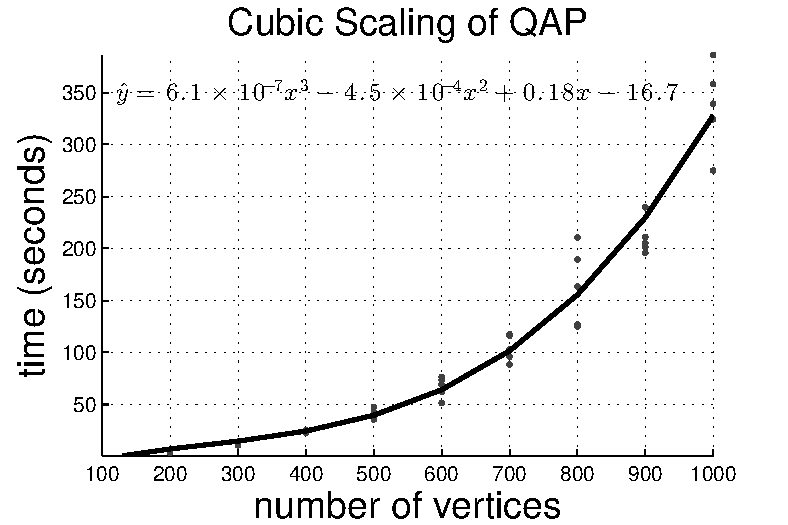
\includegraphics[width=1.0\linewidth]{../figs/ErdosRenyi_results.pdf}
	\caption{Running time of \FAQ as function of number of vertices. Data was sampled from an Erd\"os-R\'enyi model with $p=log(n)/n$.  Each dot represents a single simulation, with 100 simulations per $n$.  The solid line is the best fit cubic function.  Note the leading constant is $\dot{\approx} 10^{-7}$ seconds. \FAQ the optimal objective function value in every simulation.}
	\label{fig:scaling}
\end{figure}

% subsection algorithm_complexity_and_leading_constants (end)


\subsection{QAP Undirected Benchmarks}
\label{sub:undirected}

We next assess the computational properties of \FAQ in comparison with other the previous state-of-the-art algorithms.  We therefore compare \FAQ to other approaches using a selection of the QAP benchmark library, QAPLIB \cite{Burkard1997}.  Specifically, \cite{Zaslavskiy2009} created a path following algorithm (\texttt{PATH}) based on a convex and concave relaxation of QAP.  In that manuscript, the authors considered 16 datasets from the QAPLIB benchmark, the same 16 datasets as were used in \cite{Schellewald2001}, which are known to be ``particularly difficult''.  \texttt{PATH} was shown to outperform other state-of-the-art algorithms on 14 of 16 tests.  Specifically, \texttt{PATH} was compared to the Quadratic Programming Bound approach (\texttt{QGP}) of \cite{Anstreicher2001}, the graduated assignment algorithm (\texttt{GRAD}) of \cite{Gold1996}, and Umeyama's algorithm (\texttt{U}) \cite{Umeyama1988}.  Because either \texttt{PATH} or \texttt{QBP} outperformed \texttt{GRAD} and \texttt{U} on every dataset, Table \ref{tab:1} shows the performance of \FAQ versus \texttt{PATH} and \texttt{QBP}.  \FAQ outperforms both of the previous state-of-the-art cubic algorithms on 13 out of 16 benchmarks.  Figure \ref{fig:path16} presents the same data graphically. The top panel compares both \FAQ and \texttt{PSOA}---which is the minimum of the previous state-of-the-art (either \texttt{PATH} or \texttt{QBP} here)---to the absolute minimum; \FAQ get closer than \texttt{PSOA} to the minimum on 13 of 16. The bottom panel shows the ratio of \FAQ to \texttt{PSOA}. 


\begin{table}[h!]
\caption{Comparison of \FAQ with the optimal objective function value and previous state-of-the-art on a set of 16 standard benchmarks from QAPLIB.  The best (lowest) value is in \textbf{bold}. The number of vertices for each problem is the number in its name (second column).}
\begin{center}
\begin{tabular}{|r|r|r||l|l|l|l|l|}
\hline
\# & Problem  &   Optimal   & \FAQ & \texttt{PATH} & \texttt{QBP} \\
\hline
1&    chr12c &   11156 &    \textbf{13072} &   18048 	& 20306\\
2&    chr15a &    9896 &    27584 &   \textbf{19086} 	& 26132\\
3&    chr15c &    9504 &    \textbf{11936}  &   16206 	& 29862\\
4&   chr20b &    2298 & \textbf{3068} &    5560 		& 6674\\
5&    chr22b &    6194 &    \textbf{8482} &    8500 		& 9942\\
6&    esc16b & 292 &    320 & 300 		& \textbf{296}\\
7& rou12 &  235528 &    \textbf{253684} &  256320 	& 278834\\
8& rou15 &  354210 &    \textbf{371458} &  391270 	& 381016\\
9& rou20 &  725522 &    \textbf{743884} &  778284 	& 804676\\
10&    tai10a &  135028 &   157954 &  \textbf{152534} 	& 165364\\
11&    tai15a &  388214 &   \textbf{397376} &  419224 	& 455778\\
12&    tai17a &  491812 &   \textbf{529134} &  530978 	& 550862\\
13&    tai20a &  703482 &   \textbf{734276} &  753712 	& 799790\\
14&    tai30a & 1818146 &  	\textbf{1894640} & 1903872 	& 1996442\\
15&    tai35a & 2422002 & 	\textbf{2460940} & 2555110 	& 2720986\\
16&    tai40a & 3139370 &  	\textbf{3227612} & 3281830 	& 3529402\\
    \hline
\end{tabular}
\end{center}
\label{tab:1}
\end{table}%


\begin{figure}[htbp]
	\centering
		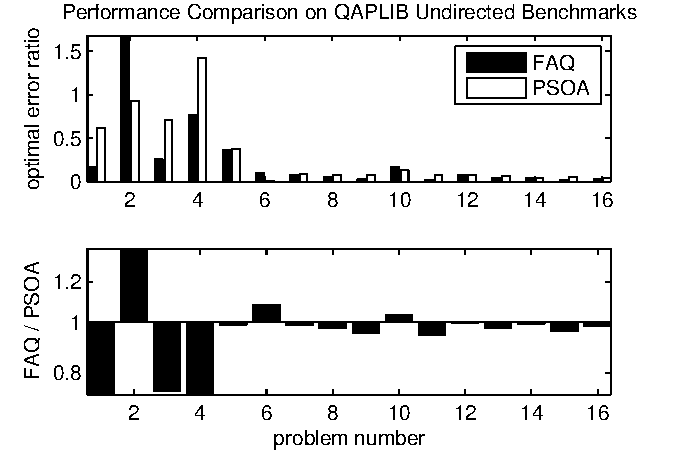
\includegraphics[width=1.0\linewidth]{../figs/path16.pdf}
	\caption{Performance of \FAQ relative to the previous state-of-the-art (\texttt{PSOA}) algorithms on the undirected QABLIB benchmarks.  Top: The optimal error ratio is defined: $(\mh{f} - f^*)/f^*$, for $\mh{f}$ being the minimum function value found by each algorithm, and $f^*$ is the optimal (minimum) value.  Bottom: Ratio of \FAQ minimum to \texttt{PSOA} minimum.  Note that both panels indicate that \FAQ gets closer to the minimum on 13 of 16 benchmarks.}
	\label{fig:path16}
\end{figure}


\subsection{QAP Directed Benchmarks}
\label{sub:directed}

Nothing in the development of our algorithm depends on the graphs being simple; indeed, \FAQ applies equally well to directed graphs.  To assess the performance of \FAQ on directed graphs, we compare the performance of our algorithm to the previous state-of-the-art. Liu et al.  recently developed an extended path following algorithm for directed graphs \cite{Liu2012}. They compare the performance of their algorithm (\texttt{EPATH}) with several other algorithms on a set of 16 benchmarks from QAPLIB.  In particular, they consider \texttt{U} and \texttt{GRAD}, as well as an algorithm called \texttt{QCV}, which solves a convex relaxation similar to our approach.  The \texttt{EPATH} algorithm achieves at least as low objective value as the other algorithms on 15 of 16 benchmarks.  Our algorithm, \texttt{FAQ}, always gets the best of the five algorithms.  Table \ref{tab:directed} shows the numerical results comparing \FAQ to \texttt{EPATH} and \texttt{GRAD}, which sometimes did better than \texttt{EPATH}.  Note that some of the algorithms achieve the absolute minimum on some benchmarks.  Figure \ref{fig:lipa16} compares \FAQ to whichever other algorithm did best, clearly indicating that \FAQ is the best on these benchmarks.


\begin{table}[h!]
\caption{Comparison of \FAQ with optimal objective function value and previous state-of-the-art for undirected graphs.  The best (lowest) value is in \textbf{bold}. Asterisks indicate achievement of the global minimum.  The number of vertices for each problem is the number in its name (second column).}
\begin{center}
\begin{tabular}{|r|r|r||l|l|l|l|l|}
	\hline 
	          \# &  Problem &      Optimal & \texttt{FAQ} & \texttt{EPATH} & \texttt{GRAD} \\
	\hline 
	           1 &  lipa20a &     3683 & \textbf{3791} &     3885 &     3909 \\ 
	           2 &  lipa20b &    27076 & \textbf{27076}$^*$ &    32081 &    \textbf{27076}$^*$ \\ 
	           3 &  lipa30a &    13178 & \textbf{13571} 	&    13577 &    13668 \\ 
	           4 &  lipa30b &   151426 & \textbf{151426}$^*$ & \textbf{151426}$^*$ &   \textbf{151426}$^*$ \\ 
	           5 &  lipa40a &    31538 & \textbf{32109} 	&    32247 &    32590 \\ 
	           6 &  lipa40b &   476581 & \textbf{476581}$^*$ &   \textbf{476581}$^*$ &   \textbf{476581}$^*$ \\ 
	           7 &  lipa50a &    62093 & \textbf{62962} &    63339 &    63730 \\ 
	           8 &  lipa50b &  1210244 & \textbf{1210244}$^*$ &  \textbf{1210244}$^*$ &  \textbf{1210244}$^*$ \\ 
	           9 &  lipa60a &   107218 & \textbf{108488} &   109168 &   109809 \\ 
	          10 &  lipa60b &  2520135 & \textbf{2520135}$^*$ &  \textbf{2520135}$^*$ &  \textbf{2520135}$^*$ \\ 
	          11 &  lipa70a &   169755 & \textbf{171820} &   172200 &   173172 \\ 
	          12 &  lipa70b &  4603200 & \textbf{4603200}$^*$ &  \textbf{4603200}$^*$ &  \textbf{4603200}$^*$ \\ 
	          13 &  lipa80a &   253195 & \textbf{256073} &   256601 &   258218 \\ 
	          14 &  lipa80b &  7763962 & \textbf{7763962}$^*$ &  \textbf{7763962}$^*$ &  \textbf{7763962}$^*$ \\ 
	          15 &  lipa90a &   360630 & \textbf{363937} &   365233 &   366743 \\ 
	          16 &  lipa90b & 12490441 & \textbf{12490441}$^*$ & \textbf{12490441}$^*$ & \textbf{12490441}$^*$ \\ 
	\hline
	\end{tabular}
\end{center}
\label{tab:directed}
\end{table}%


\begin{figure}[htbp]
	\centering
		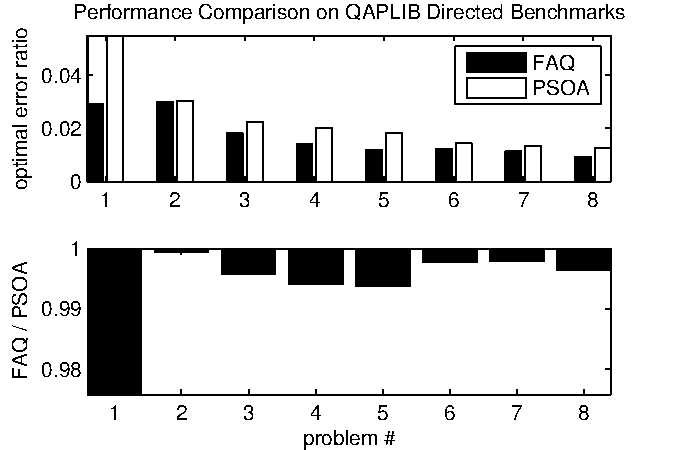
\includegraphics[width=1.0\linewidth]{../figs/lipa16.pdf}
	\caption{Performance of \FAQ relative to the previous state-of-the-art (\texttt{PSOA}) algorithms on the undirected QABLIB benchmarks. Top and Bottom panels as in Figure \ref{fig:path16}.  Note that \FAQ gets closer to the minimum on all 8 benchmarks for which the \FAQ and \texttt{PSOA} answer differ.}
	\label{fig:lipa16}
\end{figure}



\subsection{rQAP solves QAP in certain special cases} % (fold)
\label{sub:rqap_solves_qap_}

The above numerical results can be strengthened by the below theoretical results.  
Note that rQAP relaxes the constraints of Eq. \eqref{eq:trQAP}, which suggests that in certain important special cases, the minimum of rQAP will be identical to the minimum of QAP. On the other hand, the equality between Eq. \eqref{eq:trQAP2} and Eq. \eqref{eq:trQAP} follows from dropping cross-terms that fall out of the optimization because $P$ is constrained to be a permutation matrix.  If we had relaxed the constraints prior to canceling those terms, this equality would not follow.  This leads us to wonder in which circumstances are the objective functions of QAP and rQAP equal.  The following lemma clarifies:
 % This insight leads to the following theorem:
% Although, rLAP and LAP are always equivalent, in general, it is not the case that FAQ and QAP are equivalent.  However, in a certain important special case, FAQ and QAP are equivalent.
\begin{lem}
	If $A$ and $B$ are the adjacency matrices of simple graphs (symmetric, hollow, and binary) that are isomorphic to one another, then the minimum of rQAP is equal to the minimum of QAP.
\end{lem}
\begin{proof}
Because any feasible solution to QAP is also a feasible solution to rQAP, we must only show that the optimal objective function value to rQAP can be no better than the optimal objective function value of QAP.  Let $A=PBP\T$, so that $\langle A, PBP\T\rangle=2m$, where $m$ is the number of edges in $A$.  If rQAP could achieve a lower objective value, then it must be that there exists a $D \in \mc{D}$ such that $\langle A, DBD\T\rangle > \langle A, PBP\T\rangle = 2m$ (remember that we are minimizing the negative Euclidean inner product). For that to be the case, it must be that $(DBD\T)_{ij} \geq 1$ for some $(u,v)$.  That this is not so may be seen by the submultiplicativity of the norm induced by the $\ell_{\infty}$ norm:
$\norm{Dx}_\infty \leq \norm{D}_{\infty,\infty} \norm{x}_\infty$.  Applying this twice (once for each doubly stochastic matrix multiplication) yields our result.
% Consider $d_i=\langle D, \text{col}_i(BD\T) \rangle$, where $\text{col}_i(\cdot)$ indicates the $i^{th}$ column of the matrix.  $d_i \leq 1$ for all $i \in [n]$, therefore, our result holds.
\end{proof}
% subsection rqap_solves_qap_ (end)


% section theoretical_results (end)

% \section{Numerical Results} % (fold)
% \label{sub:numerical_results}


% subsection numerical_results (end)


\subsection{Multiple Restarts} % (fold)
\label{sub:multiple_restarts}

Although \FAQ outperformed \texttt{PSOA} on 13 of 16 undirected benchmarks, and always did the best amongst 16 of 16 directed benchmarks, it was annoying to us that we did not do best on all 32 benchmarks.  
% Note that the computational bottleneck of both \FAQ and \texttt{PATH} is the Hungarian algorithm which solves a LAP. 
% \FAQ strives to solve a non-convex problem.
% In \texttt{PATH}, the algorithm finds the minimum of a convex path between two extremes, $F_0$ and $F_1$.  Similarly, \texttt{QBP} finds the minimum of a convex program.  Our approach, on the other hand, does not construct a convex problem to solve, rather, it chooses an initial starting point and then finds a local optimum (note that the initial position of the \texttt{PATH} algorithm could also be variable, because $F_0$ is not convex as they assert, so their starting point depends on their initialization). 
% 
We utilize the non-convexity of rQAP is as a feature, although it can equally well be regarded as a bug  (because rQAP is non-convex so the solution found by \FAQ depends on the initial condition).  It is a feature, however, if (i) we have some reason to believe that better solutions exist (many algorithms efficiently compute relatively tight lower bounds \cite{Anstreicher2009}), and (ii) we can efficiently search the space of initial conditions.  Although we  lack any supporting theory of optimality, we do know how to sample feasible starting points.  Specifically, we desire that our starting points are ``near'' the flat matrix, and satisfy the conditions.  Therefore, we  sample $K \in \mc{D}$, a random doubly stochastic matrix using 10 iterations of Sinkhorn balancing \cite{Sinkhorn1964}, and let our initial guess be $P^{(0)}=(J+K)/2$, where $J$ is the doubly flat matrix.  We can therefore use any number of restarts with this approach.  

Table \ref{tab:2} shows the performance of running \FAQ 3 and 100 times, reporting only the best result (indicated by \texttt{FAQ}$_3$ and \texttt{FAQ}$_{100}$, respectively), and comparing it to the best performing result from Table \ref{tab:1}.  It only required three restarts to outperform all other cubic algorithms on all 16 of 16 benchmarks.  Moreover, after 100 restarts, \FAQ finds the absolute minimum on 3 of the 16 benchmarks. Figure \ref{fig:restarts} graphically demonstrates these results. 
 Note that restarting \FAQ a fixed number of multiple times is still cubic.  Future work could investigate performance as a function of the number of restarts. %, although with an arbitrary number of random restarts, stating that it is cubic is somewhat meaningless.  



\begin{table}[h!]
\caption{Comparison of \FAQ with optimal objective function value and the best result from Table \ref{tab:1} on undirected benchmarks.  Note that \FAQ restarted 100 times finds the optimal objective function value in 3 of 16 benchmarks, and that \FAQ restarted 3 times finds a minimum better than the PSOA on all 16 benchmarks.}
\begin{center}
\begin{tabular}{|r|r|r||l|l|l|l|l|}
\hline
\# & Problem  &   Optimal    & \texttt{FAQ}$_{100}$ & \texttt{FAQ}$_{3}$ & min(\FAQ,\texttt{PSOA}) \\
\hline
1&    chr12c &   11156 &    \textbf{12176} &   13072 & 13072 \\
2&    chr15a &    9896 &    \textbf{9896}$^*$ &   17272 &  19086 \\
3&    chr15c &    9504 &    \textbf{10960} &   14274 &  16206 \\
4&   chr20b &    2298 &     \textbf{2786} &    3068 &    3068 \\
5&    chr22b &    6194 &    \textbf{7218} &    7876 &   8482 \\
6&    esc16b & 	292 & 		\textbf{292}$^*$ & 294 &    296 \\
7& 	   rou12 &  235528 &  \textbf{235528}$^*$ &  238134 &    253684 \\
8& 	   rou15 &  354210 &  \textbf{356654} &  371458 &    371458 \\
9&      rou20 &  725522 &  \textbf{730614} &  743884 &    743884 \\
10&    tai10a &  135028 &  \textbf{135828} &  148970 &    152534 \\
11&    tai15a &  388214 &  \textbf{391522} &  397376 &    397376 \\
12&    tai17a &  491812 &  \textbf{496598} &  511574 &    529134 \\
13&    tai20a &  703482 &  \textbf{711840} &  721540 &    734276 \\
14&    tai30a & 1818146 & \textbf{1844636} & 1890738 &  1894640 \\
15&    tai35a & 2422002 & \textbf{2454292} & 2460940 &  2460940 \\
16&    tai40a & 3139370 & \textbf{3187738} & 3194826 &  3227612 \\
    \hline
\end{tabular}
\end{center}
\label{tab:2}
\end{table}%

\begin{figure}[htbp]
	\centering
		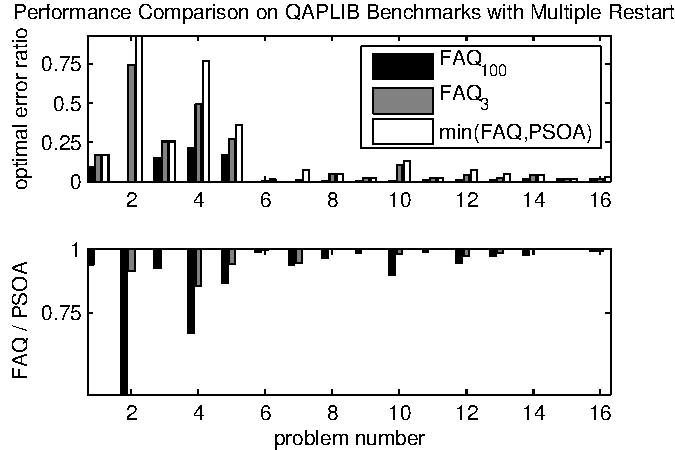
\includegraphics[width=1.0\linewidth]{../figs/path16_restarts.pdf}
	\caption{Performance of \FAQ with multiple restarts on the undirected benchmarks.}
	\label{fig:restarts}
\end{figure}


% subsection multiple_restarts (end)

% 
% \begin{figure}[htbp]
% 	\centering			
% 	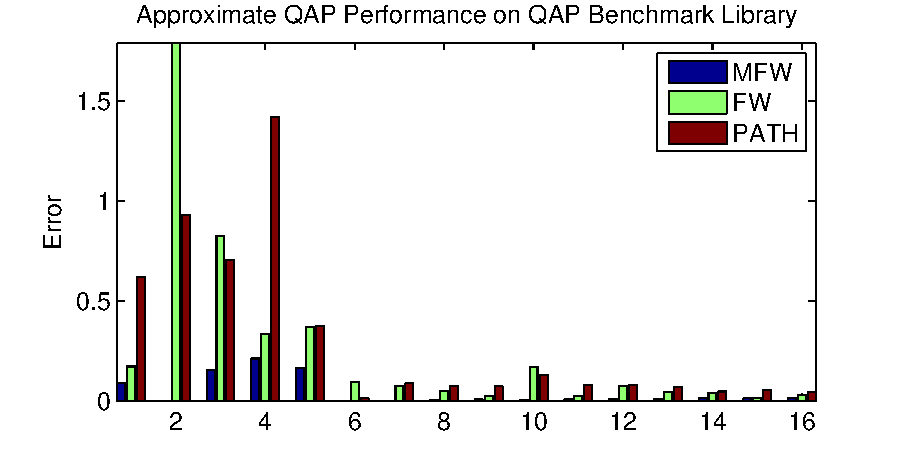
\includegraphics[width=1.0\linewidth]{../figs/benchmarks.pdf}
% 	\caption{\texttt{FAQ}$_3$ outperforms the previous state-of-the-art (PSOA) on all 16 benchmark graph matching problems.  Moreover, \FAQa outperforms PSOA on 12 of 16 tests.  For 3 of 16 tests, \FAQb achieves the minimum (none of the other algorithms ever find the absolute minimum), as indicated by a black dot.  Let $f_*$ be the minimum and $\mh{f}_x$ be the minimum achieved by algorithm $x$.  Error is $\mh{f}_x/f_*-1$.  }
% 	\label{fig:fwpath}
% \end{figure}



\subsection{Brain-Graph Matching} % (fold)
\label{sub:connectome_classification}

A ``connectome'' is a brain-graph in which vertices correspond to (collections of) neurons, and edges correspond to connections between them. The \emph{Caenorhabditis elegans} (\emph{C. elegans}) is a small worm (nematode) with $302$ labeled vertices.  We consider the subgraph with $279$ somatic neurons that form edges with other neurons \cite{WhiteBrenner86, Varshney2011}.  Two distinct kinds of edges exist between vertices: chemical and electrical ``synapses'' (edges). Any pair of vertices may have several edges of each type. Moreover, some of the synapses are hyper-edges amongst more than two vertices.   Thus, the connectome of a \emph{C. elegans} may be thought of as a weighted multi-hypergraph, where the weights are the number of edges of each type.  \FAQ natively operates on weighted or unweighted graphs.  We therefore conducted the following synthetic experiments.  

Let $A_{ij;z} \in \{0,1,2,\ldots\}$ be the number of synapses from neuron $i$ to neuron $j$ of type $z$ (either chemical $c$ or electrical $e$), and let $A_z=\{A_{ij;z}\}_{i,j \in [279]}$ for $z \in \{e,c\}$ correspond to the electrical or chemical connectome.  To generate synthetic data, we let $B_z^{(k)}=Q_z^{(k)} A_z {Q_z^{(k)}}\T$, for some $Q_z^{(k)}$ chosen uniformly at random from $\mc{P}$, effectively shuffling the vertex labels of the connectome.  Then, we try to graph match $A_z$ to $B_z^{(k)}$, for $z \in \{e,c\}$ and for $k =1,2,\ldots, 10$, that is, we repeat the experiment 100 times.  We define accuracy as the fraction of vertices correctly assigned. We always start with the doubly flat matrix.
% by the value of our objective function, $f(P_z^{(k)})$.  
% To evaluate the impact of multiple restarts, for both connectomes, we restarted \FAQ up to 30 times.   Specifically, our stopping criteria on the number of restarts was either (i) perfect assignment or (ii) 30 restarts.

% Table \ref{tab:1} shows the mean (standard deviation) of accuracy and solution time for both connectomes.  For the chemical connectome, \FAQ always found the optimal solution, but not so for the electrical connectome.  


\begin{figure}[htbp]
	\centering
		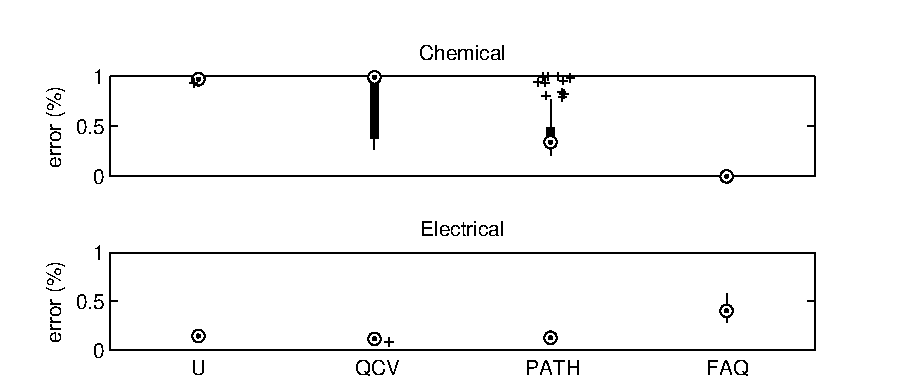
\includegraphics[width=1.1\linewidth]{../figs/connectomes.pdf}
	\caption{Performance of \texttt{U}, \texttt{QCV}, \texttt{PATH}, and \FAQ on synthetic C.~elegans connectome data.  Error is the fraction of vertices correctly matched.  Circle indicates the median, thick black bars indicate the quartiles, thin black lines indicate extreme but non-outlier points, and plus signs are outliers. For the chemical connectome, \FAQ always obtained the optimal solution, whereas none of the other algorithms ever found the optimal.  On the other hand, for the electrical connectome, none of the algorithms ever found the optimal.}
	\label{fig:connectomes}
\end{figure}


Figure \ref{fig:connectomes} displays the results of \FAQ along with three previous state-of-the-art algorithms on the two connectomes: (i) Umeyama's algorithm\texttt{U}, (ii) a quadratic convex relaxation \texttt{QCV} (which follows from relaxing the permutation matrix constraint to the doubly stochastic constraint in Eq. \eqref{eq:trQAP2}), and (iii) \texttt{PATH}.  The top left panel indicates that \FAQ \emph{always} found the optimal solution for the chemical connectome, whereas none of the other algorithms \emph{ever} found the optimal solution.  On the other hand, the top right panel shows that for the electrical connectome, none of the four algorithms ever found the optimal. One hundred restarts of \FAQ failed to significantly improve the results. 

The bottom panels compare the wall time of the various algorithms, running on an 2.2 GHz Apple MacBook. Note that we have only a Matlab implementation of \texttt{FAQ}, whereas the other algorithms are implemented in C.  Nonetheless, \FAQ runs nearly as quickly as both \texttt{U} and \texttt{QCV}, and significantly faster than \texttt{PATH}, for both connectomes.  %This suggests that lower level language implementation of \FAQ might be 

 % \FAQ ran very quickly, finding the optimal solution for the chemical connectome and converging for the electrical connectome, in only a few seconds.  Although computer times are not directly comparable, as our \FAQ implementation is in Matlab, and the other algorithms are coded in C, consider \FAQ versus \texttt{PATH}.  The bottleneck in both is \texttt{FW}.  In \texttt{PATH}, the number of \texttt{FW}s depends on a parameter, $d\lambda$, which sets the step size along the path. The \texttt{PATH} paper, \cite{Zaslavskiy2009}, describes an adaptive scheme for updating $d\lambda$, with a lower bound of $10^{-5}$, clearly indicating that sometimes, \texttt{FW} is run many times.  On the other hand, in \texttt{FAQ}, \texttt{FW} is always run only once.  

The properties of these connectomes are analyzed in \cite{Varshney2011}; a cursory evaluation of the properties of these graphs does not suggest to us why the chemical connectome was so much easier to graph match than the electrical one. 


To investigate the performance of \FAQ on undirected graphs, we ran \FAQ on binarized symmeterized versions of the graphs ($A_{ij;z}=1$ if and only if $A_{ij;z}\geq 1$ or $A_{ji;z} \geq 1$).  The resulting errors are nearly identical to those presented in Figure \ref{fig:connectomes}, although speed increased by greater than a factor of two. Note that the number of vertices in this brain-graph matching problem---279---is several times larger than the largest of the 32 benchmarks used above. 




\section{Discussion}
\label{sec:discussion}

This work presents a fast approximate quadratic assignment problem algorithm called \FAQ for approximately solving large graph matching problems, motivated by brain-graphs.  Our key insight was to relax the binary constraint of QAP to its continuous and non-negative counterpart---the doubly stochastic matrix---which is the convex hull of the original feasible region.  
Numerically, we demonstrated that not only is \FAQ cubic in time, but also its leading constants are quite small, suggesting that it might scale up reasonably well.  Moreover, it achieves better performance than previous state-of-the-art cubic-time algorithms on 29 of the 32 standard QAP benchmarks, including both directed and undirected graph matching problems.  Because rQAP is non-convex, we also consider multiple restarts, and achieve improved performance for the remaining three benchmarks using only two or three restarts.  We then demonstrate that the solution to our relaxed optimization problem, rQAP, is identical to that for QAP whenever the two graphs are simple and isomorphic to one another.  Finally, we used it to match C.~elegans connectomes to permuted versions of themselves. For the chemical connectome, of the four state-of-the-art algorithms, \FAQ achieved perfect performance $100\%$ of the time, whereas none of the other three algorithms ever achieved perfect performance. On the other hand, all the algorithms struggled with the electrical connectome.   Note that these connectomes have 302 vertices, significantly more than all the benchmarks. 

% our motivating application: brain-graph matching.  \FAQ solved a brain-graph matching problem, which has an order of magnitude more vertices than any of the 16 QAP benchmarks.

% These insights led to an approximate QAP solver with a few distinct features. %While others have incorporated the FW algorithm as a subroutine of a graph matching strategy \cite{Zaslavskiy2009}, we modified the FW algorithm for GM in a few ways.  

% First, after finding a local solution to the relaxed problem, we project the resulting doubly stochastic matrix onto the set of permutation matrices.  Second, we initialize the algorithm using either the identity matrix or the doubly flat matrix (the matrix where all elements are $1/n$).  These choices seem to us to be the most obvious places to start if one must choose.  Third, if one of those choices does not work, we restart FW with other ``nearby'' initial points.  These modifications facilitate improved performance on \emph{all} the benchmarks we considered.  Moreover, although the algorithm scales cubically with the number of vertices, the leading constants are very small ($\mc{O}(10^{-7})$ seconds), so the algorithm runs quite fast on reasonably sized networks (e.g., $n \dot{\approx} 100$).  Indeed, on a biologically inspired GM problem, \emph{C. elegans} connectome mapping, this approach was both fast and effective.  

Fortunately, our work is not done. Even with very small leading constants for this algorithm, as $n$ increases, the computational burden gets quite high.  For example, extrapolating the curve of Figure \ref{fig:scaling}, this algorithm would take about 2 years to finish (on a standard laptop from 2011) when $n=20,000$.  We hope to be able to approximately solve rQAP on graphs much larger than that, given that the number of neurons in even a fly brain, for example, is $\mc{O}(10^5)$.  Therefore, more efficient implementations are of interest.  

% Although \FAQm consistently found the optimal solution for the \emph{C. elegans} chemical connectome, connectomes for different organisms even within a species are unlikely to be identical. Even if all connectomes of a particular species were identical, measurement error will likely persist \cite{Helmstaedter2011}. Therefore, \texttt{FAQ}$_m$'s scientific utility will largely rest on its performance under noisy conditions, which we aim to explore in future work.  

Additional future work might generalize \FAQ in a number of ways.  First, many (brain-) graphs of interest will be errorfully observed \cite{Priebe2011}, that is, vertices might be missing and putative edges might exhibit both false positives and false negatives.  Explicitly dealing with this error source is both theoretically and practically of interest \cite{VP11_unlabeled}.  
% that QAP and LAP are so similar suggests that perhaps one could simply implement a single iteration of QAP starting from the identity.  While not changing the order of complexity, it could reduce computational time by at least an order of magnitude, without drastically changing performance properties (because convergence typically requires around $5-15$ iterations for the graphs we tested).  The relative performance/computational cost trade-off merits further theoretical investigations.  
Second, for many brain-graph matching problems, the number of vertices will not be the same across the brains.  Recent work from \cite{Zaslavskiy2009, Zaslavskiy2010} and \cite{Escolano2011} suggest that extensions in this direction would be both relatively straightforward and effective. Third, the most ``costly'' subroutine is LAP.  Fortunately, LAP is a quadratic optimization problem with linear constraints.  A number of parallelized optimization strategies could therefore potentially be brought to bear on this problem \cite{Boyd2011}.  Fourth, our matrices have certain special properties, namely sparsity, which makes more efficient algorithms (such as ``active set'' algorithms) readily available for further speed increases.  Fourth, for brain-graphs, we have some prior information that could easily be incorporated in the form of vertex attributes.  For example, position in the brain, cell type, etc., could be used to measure ``dissimilarity'' between vertices.  %The WGMP could easily incorporate these dissimilarities, in fact, the original QAP formulation already encodes them via the matrix $C$; that matrix was simply dropped when WGMP was originally proposed.  
% The objective function could then be modified to give
% \begin{align} \label{eq:Jqap}
% 	\mt{Q}_{AB}= \argmin_{Q \in \mc{D}} \norm{Q A Q\T - B}^2_F + \lambda J(Q),
% \end{align}
% where $J(Q)$ is a dissimilarity based penalty and $\lambda$ is a hyper-parameter.  
Finally, although this approach natively operates on both unweighted and weighted graphs, multi-graphs are a possible extension.

In conclusion, this manuscript has presented an algorithm for approximately solving the quadratic assignment problem that is fast, effective, and easily generalizable.  Yet, the $\mc{O}(n^3)$ complexity remains too slow to actually solve our problems of interest.  To facilitate further development and applications, all the code and data used in this manuscript is available from the first author's website, \url{http://jovo.me}.

% \subsection{Related Problems} % (fold)
% \label{sub:related_problems}
% 
% In addition to brain-graph matching, large approximate graph matching could be fruitful for a number of other domains.  For example, consider social networks.  In both the Twitter and Facebook graph, each vertex represents an individual.  For many users of each social networking application, it is not clear whether they have an account on another social network, and if so, what is the label of that account.  Thus, graph matching in this domain could suggest assignments of Facebook user names to twitter accounts.  Alternately, consider a language graph, where each vertex represent a word in some language, and an edge represent the existence of an adjacency between a pair of words in a text corpus of that language.  If one could match a pair of graphs corresponding to two different languages, one might obtain a highly effective machine translation tool. This might be especially true when no additional information is known about one or both languages.
% 
% Consider the scale of these problems.  Twitter and Facebook have $\mc{O}(10^8)$ users and languages often have $\mc{O}(10^5)$ words.  Exact graph matching algorithms require exponential time in the worst case.  So, even considering the smallest problem above, brain-graph matching, the fastest exact graph matching algorithms would require more time than there are nanoseconds since the big bang.\footnote{Assuming the big bang occurred 15 billion years ago means about $10^{17}$ seconds ago.  Assuming computational time is $1.004^n$ nanoseconds, even when $n=10^4$, the problem will already exceed the number of seconds since the big bang} This motivates us to consider developing \emph{approximate} (or \emph{heuristic}) algorithms, with polynomial time complexity.  Indeed, we present here an algorithm the requires approximately one week on a standard desktop computer (running non-optimized code) to match graphs with $\mc{O}(10^4)$ vertices.
% 
% 
% % subsection related_problems (end)


\appendix

% \textbf{APPENDIX}
\section{Linear Assignment Problems} % (fold)
% \label{ssub:linear_assignment_problems}

% subsubsection linear_assignment_problems (end)

The standard way of writing a Linear Assignment Problem (LAP) is
\begin{subequations} \label{eq:LAP}
\begin{align}
	 \text{(LAP) }\quad  &\underset{\pi}{\text{minimize}} \sum_{u,v \in [n]} a_{u \pi(v)} b_{ij} \\
	&\text{subject to } \pi \in \Pi,
\end{align}
\end{subequations}
which can be written equivalently in a number of ways using the notion of permutation matrix introduced in the main text:
\begin{subequations} \label{eq:LAP2}
\begin{align}
	&\argmin_{\PmcP} \norm{PA - B}_F =\\
	&\argmin_{\PmcP} \, tr(PA-B)\T (PA-B)=\\ 
	% &\argmin_{\PmcP} tr (A\T P\T PA) - tr(2PAB\T) + tr(B\T B)=\\ 
	&\argmin_{\PmcP}  -tr (P AB\T) = \argmin_{\PmcP}  -\langle P\T, AB\T \rangle = \label{eq:2c} \\
	% &\argmin_{\PmcP}  -\sum_{u,v \in [n]} p_{ij} a_{ij} b_{ji}
	% =\\% &\argmin_{\PmcP}  - \text{vec}(P)\T \text{vec}(AB\T).=\\
	&\argmin_{\PmcP}  -\langle P, AB\T \rangle, \label{eq:dotLAP}
\end{align}
\end{subequations}
where $\langle \cdot,\cdot \rangle$ %the equality on the second to last line defines 
is the usual Euclidean inner product, i.e., $\langle X,Y\rangle \defn tr(X\T Y)= \sum_{ij} x_{ij} y_{ij}$.
While the objective function and the first two constraints of LAP are linear, the binary constraints make solving even this problem computationally tricky.  Nonetheless, in the last several decades, there has been much progress in accelerating algorithms for solving LAPs, starting with exponential time, all the way down to $\mc{O}(n^3)$ for general LAPs, and even faster for certain special cases (e.g., sparse matrices) \cite{Jonker1987, Burkard2009}.

That Eq. \eqref{eq:dotFW1} is a LAP is evident by considering Eq. \eqref{eq:dotLAP}.  If $A=\nabla_P^{(i)}$ and $B=I$ (the $n\times n$ identity matrix), then Eq. \eqref{eq:dotFW1} is identical to Eq. \eqref{eq:dotLAP}.


% The last form indicates that LAP is a linear programming problem (hence the name).  Yet, the constraints, $\mc{P}$, make it a bit trickier.  The feasible region $\mc{P}$ can be written as a set of three constraints: two linear equality constraint sets and a binary constraint.  The LAP objection function with constraints can explicitly be written:
% \begin{align}
% 		&\text{minimize}_P  &&\sum_{u \in \mc{V}} -p_{ij} a_{ij} b_{ji} \nonumber \\
% 		&\text{subject to } && \sum_{u \in \mc{V}} p_{ij} = 1 \, \forall u \in \mc{V} \nonumber \\
% 		& && \sum_{v \in \mc{V}} p_{ij} = 1 \, \forall v \in \mc{V}, \nonumber \\
% 		& &&p_{ij} \in \{0,1\} \, \forall u,v. \label{eq:rLAP}	
% \end{align}
% Perhaps because LAP comes up in a wide variety of contexts, a large number of algorithms have been developed to solve LAP \cite{Burkard2009}.  These algorithms have become increasing efficient.  
% One of the most popular algorithms, the so-called ``Hungarian algorithm'' has time complexity $\mc{O}(n^3)$ \cite{Jonker1987}.  Under certain conditions (for example, when $AB\T$ is sparse), faster implementations are also available.  As will be seen below, LAP is a key subroutine to our inexact QAP solution.  

To solve a LAP, consider a continuous relaxation of LAP, specifically, relaxing the permutation matrix constraint to a doubly stochastic matrix constraint:
% A matrix $P$ is doubly stochastic precisely when $P$ satisfies the following three conditions: 
% \begin{enumerate}
% \item	$P\mb{1} = \mb{1}$,
% \item	$P\T \mb{1}=\mb{1}$, %\\
% \item 	$P \in  \Real_+^{n \times n}$,
% \end{enumerate}
% where the third constraint relaxes the binary constraints of the permutation matrices with a non-negativity constraint.  
% Let $\mc{D}$ be the set of doubly stochastic matrices.
% With this, we now state a relaxed LAP problem:
\begin{subequations} \label{eq:rLAP}
\begin{align}
		\text{(rLAP) } \quad &\underset{P}{\text{minimize}}  &&-\langle P, AB\T \rangle \\
		&\text{subject to } && P \in \mc{D}.
		% && \sum_{u \in \mc{V}} p_{ij} = 1 \, \forall u \in \mc{V} \nonumber \\
		% 		& && \sum_{v \in \mc{V}} p_{ij} = 1 \, \forall v \in \mc{V}, \nonumber \\
		% 		& &&p_{ij} \geq 0 \, \forall u,v, \label{eq:ALAP}	
\end{align}
\end{subequations}
As it turns out, solving rLAP is equivalent to solving LAP.
\begin{prop}
	LAP and rLAP are equivalent, meaning that they have the same optimal objective function value.
\end{prop}
\begin{proof}
	Although this proposition is typically proven by invoking total unimodularity, we present a simpler proof here.	Let $P'$ be a solution to LAP and let $P = \sum_{i\in[k]} \alpha_i P^{(i)}$ be a solution to rLAP for some positive integer $k$, permutation matrices $\{P^{(i)}\}_{i \in [k]}$, and positive real numbers $\{\alpha_i\}_{i \in[k]}$ such that $\sum_{i \in [k]} \alpha_i=1$.  Note that 
	\begin{align*}
	\langle P,AB\T \rangle &= \langle  \sum_{i\in[k]} \alpha_i P^{(i)}, AB\T \rangle=  \sum_{i\in[k]} \alpha_i \langle  P^{(i)}, AB\T \rangle	 \\
	&\leq \sum_{i\in[k]} \alpha_i \langle P', AB\T  \rangle = \langle P', AB\T \rangle \leq \langle P, AB\T \rangle,
	\end{align*}
	% then we have a contradiction, 
	because $P'$ is feasible in rLAP.
	\end{proof}
This relaxation motivates our approach to approximating QAP.

	



% use section* for acknowledgement
\ifCLASSOPTIONcompsoc
  % The Computer Society usually uses the plural form
  \section*{Acknowledgments}
\else
  % regular IEEE prefers the singular form
  \section*{Acknowledgment}
\fi

The authors would like to acknowledge two helpful reviewers as well as Lav Varshney for providing the data.
% This work was partially supported by the Research Program in Applied Neuroscience. 

% Can use something like this to put references on a page
% by themselves when using endfloat and the captionsoff option.
\ifCLASSOPTIONcaptionsoff
  \newpage
\fi

\bibliography{/Users/jovo/Research/other/latex/library}
\bibliographystyle{IEEEtran}

% \begin{IEEEbiographynophoto}{Joshua T. Vogelstein}
% % Joshua T. Vogelstein is a spritely young man, engulfed in a novel post-buddhist metaphor.
% 
% \end{IEEEbiographynophoto}
% 
% 
% % insert where needed to balance the two columns on the last page with
% % biographies
% %\newpage
% 
% \begin{IEEEbiographynophoto}{John C.~Conroy}
% % John C.~Conroy seems to basically always be right. He also publishes sometimes.
% 
% \end{IEEEbiographynophoto}
% 
% % \begin{IEEEbiographynophoto}{Doniell E.~Fishkind}
% % % John C.~Conroy seems to basically always be right. He also publishes sometimes.
% % 
% % \end{IEEEbiographynophoto}
% 
% \begin{IEEEbiographynophoto}{Lou Podrazik}
% 
% \end{IEEEbiographynophoto}
% 
% \begin{IEEEbiographynophoto}{Steve Kratzer}
% 
% \end{IEEEbiographynophoto}
% 
% 
% 
% \begin{IEEEbiographynophoto}{R. Jacob Vogelstein}
% % R. Jacob Vogelstein received the Sc.B. degree in neuroengineering from Brown University, Providence, RI, and the Ph.D. degree in biomedical engineering from the Johns Hopkins University School of Medicine, Baltimore, MD.  He currently oversees the Applied Neuroscience programs at the Johns Hopkins University (JHU) Applied Physics Laboratory as an Assistant Program Manager, and has an appointment as an Assistant Research Professor at the JHU Whiting School of Engineering’s Department of Electrical and Computer Engineering. He has worked on neuroscience technology for over a decade, focusing primarily on neuromorphic systems and closed-loop brain–machine interfaces. His research has been featured in a number of prominent scientific and engineering journals including the IEEE Transactions on Neural Systems and Rehabilitation Engineering, the IEEE Transactions on Biomedical Circuits and Systems, and the IEEE Transactions on Neural Networks.  
% \end{IEEEbiographynophoto}
% 
% \begin{IEEEbiographynophoto}{Carey E. Priebe}
% % Buddha in training.
% \end{IEEEbiographynophoto}
% 
% % Can be used to pull up biographies so that the bottom of the last one
% % is flush with the other column.
% % \enlargethispage{-5in}

% \documentclass[11pt]{article}
% \input{/Users/jovo/Research/other/latex/latex_document}
% 
% \title{Response to Review of TPAMI-2011-11-0845}
% \author{Vogelstein et al.}
%  
% \begin{document}
% \maketitle

\onecolumn
\setcounter{page}{1}
\section*{Response to Reviewers} % (fold)
\label{sec:response_to_reviewers}


We would like to thank the two helpful reviewers and the editor for their insightful comments.  We have extensively revised the manuscript in light of the comments we received.  Below are a few general remarks about the current revision, followed by specific responses to reviewer comments (reviewer comments are in \textbf{bold}):

\begin{itemize}
	\item  We have significantly revised the text to clarify that we have devised a fast and \emph{approximate} algorithm for solving quadratic assignment problems (QAP).  That graph matching can be cast as a QAP is useful because it ties our algorithm into a greater literature on QAP.	We were motivated to derive an approximate solution because our application of interest has between hundreds and billions of vertices, so exact algorithms are completely out of the question.  We hope that the text of this version of the manuscript conveys that sentiment clearly.  In fact, although our algorithm seems to be the best cubic-time approximate algorithm for solving graph matching problems, it is not nearly fast enough.  The incoming massive brain-graph data will hopefully motivate others to further improve on our work, which we view merely as a starting point.
	\item Our algorithm now fundamentally has an initial starting position that is fixed at the barycenter of the feasible region.  This is despite that the problem we seek to solve is non-convex, and we do not convexify it.  However, by starting at a sensible initial condition (the barycenter of the feasible region), we found that our algorithm outperforms the previous state of the art on 29 of the 32 standard benchmarks, as well as our brain-graph matching problem of interest.  
	\item Submission of this manuscript to TPAMI was motivated by our reading of the very nice paper of Zaslavskiy et al. \cite{Zaslavskiy2009}, which was recently published in TPAMI.  Zaslavskiy developed a novel PATH following algorithm, that was demonstrated to exceed the previous state of the art on 14 of 16 benchmark datasets selected from the QAP library \cite{Burkard1997}.  Although the authors of that manuscript did not explain their choice of 16, it is the exact same 16 used in a previous comparison of various approximate graph matching algorithms \cite{Schellewald2001}. Moreover, in \cite{Schellewald2001}, the authors explain that their choice of those 16 of the $>$100 datasets was based on those being ``particularly difficult''.   Our algorithm outperformed the PATH algorithm on 13 of the 16 datasets (always starting at the barycenter).  If we elect to use only 2 or 3 restarts, which we can only fruitfully do because our objective function is non-convex, we outperform all previous algorithms on all datasets we considered.
	\item Another paper was published in TPAMI while our manuscript was under review \cite{Liu2012}.  This paper extended the PATH paper to deal with directed graphs, developing an algorithm called \texttt{EPATH}.  The authors of this paper consider 16 directed benchmarks from the QAP library, and demonstrated improve performance on 15 of 16 benchmarks.  We applied our \FAQ algorithm to those same benchmarks, again always starting at the barycenter, and did at least as well or better than all previous algorithms on all 16 benchmarks.
	\item Below, we have responded in detail to the reviewers helpful comments. Reviewer comments are in bold, responses are plain text, quotes from the main text are in red.
\end{itemize}
 





% We respond to each specific comment below.

\newpage
\subsection*{Reviewer 1}

\begin{itemize}
	\item \textbf{1) A principle flaw:
	The suggested approach samples an generally NP-problem at n=1,3 or 100
	random points and search for a local minima in
	the usually highly non-convex function (the relaxed QAP).
	So, for increasing problem size the probability
	to obtain a good solution drops drastically.
	}

	In the original draft of this manuscript, we overemphasized the multiple restart aspect of this work.  In fact, our algorithm outperforms the previous state of the art cubic-time QAP algorithms on 13 of the 16 benchmarks. We have substantially revised the text to reflect this.  Specifically, in the first step of Section \ref{sec:faq}, we now write:
	
	\tr{\textbf{I: Find a suitable initial position.}  While any doubly stochastic matrix would be a feasible initial point, we choose the 
		% two choices seem natural: (i) the 
		``flat doubly  stochastic matrix,'' $J=\ve{1} \cdot \ve{1}\T/n$, which is the barycenter of the feasible region.}
	
		We have added a subsection in the results to merely remark that multiple restarts are a possibility (Section \ref{sub:multiple_restarts}). %merely commenting on the multiple restart option in a subsection. %We regrettably failed to clarify in the results that performance on the brain-graph matching task was repeated 10 times to demonstrate the repeatability of these results.

	\item \textbf{2) Insufficient evaluation:
	A report on statistical properties of the approach
	would make an evaluation of the method possible, i.e, how often
	is the best solution found by the sampling depending on the
	the problem size.
	However such information is not provided in the report.
	}
	
	
	\FAQ now always starts with the barycenter of the feasible region. Given this starting position, \FAQ outperforms the previous state-of-the-art algorithm on 29 of the 32 benchmarks considered; the particular benchmarks considered were the exact same ones used by the two most recent publications in TPAMI on graph matching \cite{Zaslavskiy2009,Liu2012}


	\item \textbf{3) Too few experiments:
	The authors have performed 16 experiments on
	the qaplib dataset which has in its standard form
	more than 100 problem instances.
	}

	We have now buttressed our results with another 16 benchmarks, the exact same benchmarks as those used in reference \cite{Liu2012} (see Section \ref{sub:directed}).  Moreover, the 16 that we used were exactly the 16 datasets used in recent TPAMI publication on the PATH algorithm for graph matching reference \cite{Zaslavskiy2009}.  Although the authors of the PATH paper did not explain their choice of 16, they are the same 16 used in reference \cite{Schellewald2001}, in which several different graph matching algorithms were compared.  In reference \cite{Schellewald2001}, it was explained that these 16 are ``particularly difficult''.  Section \ref{sub:undirected} elaborates on this in the text:
	
	\tr{
Specifically, \texttt{PATH} was compared to the Quadratic Programming Bound approach (\texttt{QGP}) of \cite{Anstreicher2001}, the graduated assignment algorithm (\texttt{GRAD}) of \cite{Gold1996}, and Umeyama's algorithm (\texttt{U}) \cite{Umeyama1988}.  Because either \texttt{PATH} or \texttt{QBP} outperformed \texttt{GRAD} and \texttt{U} on every dataset, Table \ref{tab:1} shows the performance of \FAQ versus \texttt{PATH} and \texttt{QBP}. 
	}
	
	\item \textbf{Developments reported for example in
``N. Brixius and K. Anstreicher. Solving quadratic assignment problems
using convex quadratic programing relaxations. Optimization Methods
and Software.'' are completely ignored.
}


Our algorithm, like PATH, outperformed all the algorithms considered in the above mentioned citation.  We have now clarified this in Section \ref{sub:directed}:

	\tr{
\FAQ outperforms both of the previous state-of-the-art inexact cubic algorithms on 13 out of 16 benchmarks.  Figure \ref{fig:path16} presents the same data graphically. The top panel compares both \FAQ and \texttt{PSOA}---which is the minimum of the previous state-of-the-art (either \texttt{PATH} or \texttt{QBP} here)---to the absolute minimum; \FAQ get closer than \texttt{PSOA} to the minimum on 13 of 16. The bottom panel shows the ratio of \FAQ to \texttt{PSOA}. }

	\item \textbf{On a different level it seems a bit unrealistic to assume that all the
graphs they wish to compare are of equal size, however
it is not discussed or even mentioned why the authors have
reason to assume that the graphs are equally sized.}


Indeed, although for some brain-graphs the number of vertices will be the same, for many, they will not be.  We have modified Section \ref{sec:discussion} accordingly:

 	\tr{
Second, for many brain-graph matching problems, the number of vertices will not be the same across the brains.  Recent work from \cite{Zaslavskiy2009, Zaslavskiy2010} and \cite{Escolano2011} suggest that extensions in this direction would be both relatively straightforward and effective.
	}

	\item \textbf{The authors report a good performance on a quite large graph with
302 nodes, but do not indicate how the graph looks like. That
makes it difficult to speculate about reasons that make this problem
solvable by just sampling at a few positions followed by the Frank-Wolfe
algorithm. It might be that the structure of the problem is
more easy (Can the assignment be found by a spectral analysis of the
adjacency matrix?)
}

We have clarified Section \ref{sub:connectome_classification} to point out extensive analyses of the brain-graphs by reference \cite{Varshney2011}:

	\tr{
The properties of these connectomes are analyzed in \cite{Varshney2011}; a cursory evaluation of the properties of these graphs does not suggest to us why the chemical connectome was so much easier to graph match than the electrical one. 	}
		

	\item \textbf{minor comments: (The line numbers at the beginning refer to both columns...)
}

Thank you, we have corrected all the minor comments.

\end{itemize}


\newpage
\subsection*{Reviewer 2}
\label{sec:reviewer_2}

\begin{itemize}
	\item \textbf{Though this is a proposal of a QAP inexact solver, it is in principle limited to graphs of the same size.}

We have now mentioned the possibility of extending this work to deal with different numbers of vertices, and have modified the Section \ref{sec:discussion} accordingly:

	 	\tr{
Second, for many brain-graph matching problems, the number of vertices will not be the same across the brains.  Recent work from \cite{Zaslavskiy2009, Zaslavskiy2010} and \cite{Escolano2011} suggest that extensions in this direction would be both relatively straightforward and effective.	}

	\item \textbf{Even in this case, there is no reference neither experimental nor theoretical to the GA (Graduated Assignment) Algorithm (Gold and Rangarajan, PAMI'1996). }

We have now clarified in Section \ref{sub:undirected} that our algorithm outperforms the GRAD algorithm on all benchmarks tested:  

	\tr{
Specifically, \texttt{PATH} was compared to the Quadratic Programming Bound approach (\texttt{QGP}) of \cite{Anstreicher2001}, the graduated assignment algorithm (\texttt{GRAD}) of \cite{Gold1996}, and Umeyama's algorithm (\texttt{U}) \cite{Umeyama1988}.  Because either \texttt{PATH} or \texttt{QBP} outperformed \texttt{GRAD} and \texttt{U} on every dataset, Table \ref{tab:1} shows the performance of \FAQ versus \texttt{PATH} and \texttt{QBP}. 	}


% \tr{
% Because either \texttt{PATH} or \texttt{QBP} outperformed \texttt{GRAD} and \texttt{U} on every dataset, Table 1 shows the performance of \FAQ versus \texttt{PATH} and \texttt{QBP}. 
% }

	\item \textbf{This is quite simplistic when comparing to the power of deterministic annealing implicit in GA to avoid local minima. A serious comparison between both schemes should be desirable.}

Because our algorithm outperformed a previously published algorithm in TPAMI which outperformed GA (the PATH algorithm), this seemed unnecessary.

	\item \textbf{In [25] it is proposed an algorithm outperforming QBP. The method proposed here is quite similar to that in [25] (which is more focused on labeled graphs but based on FW) so I judge the proposal quite incremental.}

Indeed, our algorithm is similar to the \texttt{PATH} algorithm of reference [25] of the original, \cite{Zaslavskiy2009} in the revision.  Yet, \FAQ outperforms \texttt{PATH} on 13 of 16 benchmarks, which we believe to be significant.  Moreover, our algorithm also addressed directed graphs, while \texttt{PATH} only deals with the undirected case.  Reference  \cite{Liu2012} extends \texttt{PATH} for directed graphs, and our algorithm outperforms their \texttt{EPATH} algorithm (as well as \texttt{GRAD}, \texttt{QCV}, and \texttt{U}) on all 16 benchmarks.

	\item \textbf{See similar algorithm in ``Many-to-Many Graph Matching: a Continuous Relaxation Approach'' in 2010 (arxiv).}

Thank you for pointing out this reference, as we had not yet seen it.  Indeed, this manuscript which is contemporaneous with ours proposes a similar algorithm to \texttt{FAQ}.  However, they only consider many-to-one and many-to-many problems. Moreover, our brain-graph matching problem is unique, and motivates the development of algorithms with significantly better scaling rules.  We have modified Section \ref{sec:discussion} accordingly:

\tr{
Second, for many brain-graph matching problems, the number of vertices will not be the same across the brains.  Recent work from \cite{Zaslavskiy2009, Zaslavskiy2010} and \cite{Escolano2011} suggest that extensions in this direction would be both relatively straightforward and effective.	}


	\item \textbf{Anyway in the experiments only 16 tests where done and the analysis was focuses on the number of restarts. The proposed algorithms require 1-100 starts where in 12 of 16 it only requires 1 start (the van der Waerden matrix).}

As mentioned above, the 16 tests performed are identical to the 16 tests performed by the previous state of the art, reference [25] in the original submission (the \texttt{PATH} algorithm).  And those 16 are the same 16 as used in a previous publication testing various approximate algorithms (reference [30] in the new submission).  Moreover, the authors of [30] state that those 16 were chosen because they were ``particularly difficult''.  We have significantly rewritten the text to emphasize that our algorithm fundamentally is initialized in the barycenter of the feasible region.  A secondary point in the new submission remarks that random restarts can yield superior performance, time permitting. Section elaborates on this in the text:
	
	\tr{Specifically, \cite{Zaslavskiy2009} created a path following algorithm (\texttt{PATH}) based on a convex and concave relaxation of QAP.  In that manuscript, the authors considered 16 datasets from the QAPLIB benchmark, the same 16 datasets as were used in \cite{Schellewald2001}, which are known to be ``particularly difficult''.	}

	Moreover, we have now added another 16 benchmarks, again, the exact same benchmarks used in a previous TPAMI publication, reference \cite{Liu2012}, to evaluate performance of \FAQ on directed graphs.   \FAQ achieves a superior objective value function for all 16 benchmarks than all previous state-of-the-art algorithms, as described in Section \ref{sub:directed}.


	\item \textbf{No comments on the recently embedding methods for graph matching: see for instance: ``Graph matching through entropic manifold alignment. CVPR 2011''.
Indeed only same-size graphs seem to be explored.}


Thank you for pointing out this omission, we have rectified the text to refer to this work as mentioned above.

\end{itemize}

% section reviewer_2 (end)














% \end{document}


\end{document}



